% Provenance (never printed): see sources/outline_sources.md (Year 1: grain size and sorting;
% bedforms and sedimentary structures; fluvial, deltaic, shoreline and deep-sea deposits).
% Exercise and problem values in the Book 3 scratch calculator calc/ch21.py; figure data
% from figdata/bachelor-1/grain_size.py. Meander and delta are Book 1's (g5), sediment and
% sedimentary layer Book 1's (g7), beach Book 1's (g9); the loads, settling, the threshold
% of motion and the Hjulstrom diagram are ch. 20's; the vector mean is ch. 6's. Facies
% models and Walther's law belong to the Year 3 volume (prose pointer only). Pelagic
% sediments are ch. 22's.
\chapter{खंडजात तलछट और उनके परिवेश}\label{ch:b1:clastic-sediments}

बालू का एक मुट्ठी भर उठाकर उसे उँगलियों के बीच से बहने दीजिए: कण लगभग सब एक ही आकार के हैं, गोल और साफ़, और वे पानी की तरह बहते हैं। कुछ सौ किलोमीटर भीतर, एक पुराने हिमनद द्वारा छोड़ी गई पहाड़ी के तल पर, ज़मीन शिलाखंडों, कंकड़ों, बालू और कीचड़ का एक कड़ा, व्यवस्थाहीन मिश्रण है। दोनों निक्षेप एक ही प्रकार के मलबे से बने हैं, उन्हीं प्रकार की चट्टानों से टूटे हुए; जो उन्हें अलग करता है वह यह है कि कण कैसे चले और कहाँ आकर विश्राम में आए। एक लहर जो दिन में हज़ारों बार एक तट पर ऊपर-नीचे दौड़ती है, कणों को आकार के अनुसार छाँटती है, बारीक कणों को बहा ले जाती है और बाकियों को गोल करती है; बर्फ़ जो कुछ भी उठाती है उसे ढोती है, और पिघलने पर सब एक साथ गिरा देती है। यह अध्याय सीखता है कि ऐसी कहानियाँ कणों से ही कैसे पढ़ी जाएँ, उन संरचनाओं से जो वे नदियों और समुद्रों के तलों पर बनाते हैं, और उस क्रम से जिसमें निक्षेप एक पर एक जमे हैं।

\begin{recall}
तलछट पानी, हवा या बर्फ़ द्वारा बिछाई गई ढीली सामग्री है, और समय के साथ तलछट परतों में जमती है जो कठोर होकर तलछटी शैल बनती हैं (पुस्तक~1, कक्षा~6 और~7)। एक नदी जो अपने बाढ़-मैदान पर एक किनारे से दूसरे किनारे झूलती है, विसर्पें बनाती है; जहाँ वह समुद्र या झील में प्रवेश करके अपना भार गिराती है, वहाँ वह एक डेल्टा बनाती है; लहरें बालू को तटों पर ढेर करती हैं और तटीय धारा से उसे किनारे-किनारे खिसकाती हैं (पुस्तक~1, कक्षा~5 और~9)। एक नदी अपना भार \omterm{def:b1:erosion-transport:load}{तल-भार}, \omterm{def:b1:erosion-transport:load}{निलंबित भार} और घुले भार के रूप में ढोती है; एक कण अपने \omterm{def:b1:erosion-transport:settling}{अवसादन-वेग} से डूबता है; वह तब चलने लगता है जब \omterm{def:b1:erosion-transport:bed-shear}{तल कर्तन-प्रतिबल} उसकी \omterm{def:b1:erosion-transport:threshold}{गति की देहली} पार करता है, और \omterm{def:b1:erosion-transport:hjulstrom}{हियुलस्ट्रॉम आरेख} अपरदन, परिवहन और निक्षेपण के माध्य वेगों को \omterm{def:b1:clastic-sediments:grain-size}{कण-आकार} के विरुद्ध दिखाता है (\cref{ch:b1:erosion-transport})। दिशाओं के एक समुच्चय का सदिश माध्य उनके इकाई सदिशों के योग की दिशा है (\cref{def:b1:field-lab-methods-1:mean-orientation})।
\end{recall}

\section{कण-आकार और छँटाव}\label{sec:b1:clastic-sediments:grain-size}

एक खंडजात तलछट में, यानी पुरानी चट्टानों के टुकड़ों से बनी एक में, भूवैज्ञानिक जो पहली बात दर्ज करता है वह कणों का आकार है, क्योंकि वह उस धारा की ऊर्जा को मापता है जिसने उन्हें बिछाया। प्रकृति में \omterm{def:b1:clastic-sediments:grain-size}{कण-आकार} सात से अधिक परिमाण-कोटियों तक फैले हैं, मीटरों चौड़े शिलाखंडों से लेकर एक मिलीमीटर के हज़ारवें भाग चौड़े मृत्तिका-कणों तक, और वे अनुपातों के पैमाने पर मापे जाते हैं।

\begin{definition}[कण-आकार पैमाना, फ़ाई पैमाना]\label{def:b1:clastic-sediments:grain-size}
अवसादविज्ञान का \emph{कण-आकार पैमाना}\index{कण-आकार पैमाना} कणों के व्यासों को वर्गों में बाँटता है जिनकी सीमाएँ एक वर्ग से अगले तक दुगुनी होती हैं, \qty{1}{mm} से आरंभ करके; हर वर्ग का नाम है (बालू, गाद\ldots)। \emph{फ़ाई पैमाना}\index{फ़ाई पैमाना} एक व्यास $d$ को इस प्रकार व्यक्त करता है
\[
  \varphi = -\log_2 \frac{d}{\qty{1}{mm}},
\]
ताकि $d = 2^{-\varphi}$~mm हो: \qty{1}{mm} $\varphi = 0$ है, \qty{2}{mm} $\varphi = -1$ है, \qty{0.25}{mm} $\varphi = 2$ है, और बारीक कणों के $\varphi$ के मान बड़े हैं।
\end{definition}
% ledger: folk:udden-krumbein, folk:wentworth-classes, usgs:wentworth-phi

फ़ाई पैमाने पर \omterm{def:b1:clastic-sediments:grain-size}{कण-आकार} पैमाने का हर वर्ग एक इकाई चौड़ा है: $d$ से $2d$ तक का वर्ग $\varphi$ से $\varphi - 1$ तक जाता है। मुख्य वर्ग, सामान्य प्रयोग के नामों के साथ, \cref{tab:b1:clastic-sediments:classes} में सूचीबद्ध हैं।

\begin{table}[htbp]
\centering\small
\begin{tabular}{@{}lll@{}}
\hline
वर्ग & व्यास (\si{mm}) & $\varphi$ \\
\hline
शिलाखंड & 256 से ऊपर & $-8$ से नीचे \\
रोड़ी & 64 से 256 & $-6$ से $-8$ \\
कंकड़ & 4 से 64 & $-2$ से $-6$ \\
कणिका & 2 से 4 & $-1$ से $-2$ \\
बालू (बहुत मोटी, मोटी, मध्यम, बारीक, बहुत बारीक) & $1/16$ से 2 & 4 से $-1$ \\
गाद (मोटी, मध्यम, बारीक, बहुत बारीक) & $1/256$ से $1/16$ & 8 से 4 \\
मृत्तिका & $1/256$ से नीचे (\qty{3.9}{\micro m}) & 8 से ऊपर \\
\hline
\end{tabular}
\caption{\omterm{def:b1:clastic-sediments:grain-size}{कण-आकार} वर्ग। बालू के पाँच वर्ग हर एक एक फ़ाई इकाई चौड़े हैं, बहुत मोटी (1 से \qty{2}{mm}) से बहुत बारीक ($1/16$ से
$1/8$~mm) तक, और गाद के चार वर्ग भी वैसे ही हैं। कुछ विद्वान गाद की निचली सीमा $8\,\varphi$ के बजाय 9 रखते हैं। बजरी उन कणों का सामान्य नाम है जो \qty{2}{mm} से मोटे हैं, और कीचड़ गाद और मृत्तिका के मिश्रण का।}
\label{tab:b1:clastic-sediments:classes}
\end{table}
% ledger: folk:wentworth-classes, usgs:wentworth-phi

इस पुस्तक में शब्द \emph{मृत्तिका} के दो अर्थ हैं: यहाँ यह एक आकार-वर्ग है, और \cref{ch:b1:weathering-clays} में खनिजों का एक परिवार। अधिकांश मृत्तिका-आकार के कण \omterm{def:b1:weathering-clays:clay-mineral}{मृत्तिका-खनिज} हैं और अधिकांश \omterm{def:b1:weathering-clays:clay-mineral}{मृत्तिका-खनिज} मृत्तिका-आकार के, पर दोनों मेल नहीं खाते: बहुत बारीक पिसा क्वार्ट्ज मृत्तिका-आकार का है, और एक \omterm{def:b1:weathering-clays:clay-mineral}{कैओलिनाइट} पुस्तक गाद के आकार की हो सकती है।

\emph{आकार मापना।} बजरी को कण-कण करके कैलिपरों से मापा जाता है। बालू छानी जाती है: पूरे या आधे फ़ाई इकाई पर जालियों वाली छलनियों का ढेर हिलाया जाता है, और हर छलनी का अवशेष तौला जाता है। गाद और मृत्तिका, जो $4\,\varphi$ से बारीक हैं, अवसादन से मापी जाती हैं: तलछट पानी में घोली जाती है, और चूँकि हर कण अपने आकार से तय वेग से डूबता है (स्टोक्स का नियम, \cref{prop:b1:erosion-transport:stokes}), किसी दी गई गहराई और समय पर निलंबन में बचा द्रव्यमान बताता है कि नमूने का कितना भाग किसी दिए व्यास से बारीक है। प्रकाश के कणों द्वारा बिखराव मापने वाले लेज़र उपकरण भी अब आम हैं। परिणाम हर वर्ग में भार-प्रतिशत की एक सूची है।

\begin{definition}[माध्य कण-आकार, छँटाव]\label{def:b1:clastic-sediments:sorting}
मान लीजिए एक तलछट के \omterm{def:b1:clastic-sediments:grain-size}{कण-आकार}, फ़ाई इकाइयों में, हर वर्ग के भार से दिए वितरण वाले हैं। उसका \emph{माध्य कण-आकार}\index{माध्य कण-आकार} उस वितरण का माध्य है, और उसका \emph{छँटाव}\index{छँटाव} वितरण का प्रसार है, जो फ़ाई इकाइयों में उसके मानक विचलन से मापा जाता है: एक तलछट अच्छी तरह छँटी है जब उसके कण लगभग सब एक आकार के हों, और खराब छँटी जब वे कई वर्गों में फैले हों। दोनों या तो वर्गों के प्रतिशतों से, आघूर्ण-विधि से, या संचयी वक्र से, फ़ोक के आलेखीय मापों से परिकलित होते हैं:
\[
  M_z = \frac{\varphi_{16} + \varphi_{50} + \varphi_{84}}{3}, \qquad
  \sigma_I = \frac{\varphi_{84} - \varphi_{16}}{4} + \frac{\varphi_{95} - \varphi_{5}}{6.6},
\]
जहाँ $\varphi_p$ वह फ़ाई-आकार है जिससे मोटा नमूने का $p$ प्रतिशत है।
\end{definition}
% ledger: folk:graphic-measures

\begin{method}[छलनी-विश्लेषण से माध्य और छँटाव]\label{met:b1:clastic-sediments:graphic}
\begin{enumerate}
  \item हर वर्ग में भार-प्रतिशत $w_i$ सूचीबद्ध कीजिए, सबसे मोटे से सबसे बारीक तक, और जाँचिए कि योग \qty{100}{\percent} है (या उससे भाग दीजिए)।
  \item \emph{आघूर्ण-विधि।} $x_i$ को फ़ाई इकाइयों में वर्ग $i$ का मध्य-बिंदु लेकर, माध्य $m = \sum w_i x_i / 100$ और मानक विचलन $s = \sqrt{\sum w_i (x_i - m)^2 / 100}$ परिकलित कीजिए।
  \item \emph{आलेखीय माप।} वर्ग-सीमा से मोटे प्रतिशत प्राप्त करने के लिए प्रतिशत जोड़िए, और उन्हें $\varphi$ के विरुद्ध आलेखित कीजिए: यह संचयी वक्र है।
  \item उस पर वर्ग-सीमाओं के बीच रैखिक अंतर्वेशन से, आकार $\varphi_5$, $\varphi_{16}$, $\varphi_{50}$, $\varphi_{84}$ और $\varphi_{95}$ पढ़िए।
  \item $M_z$ और $\sigma_I$ परिकलित कीजिए (\cref{def:b1:clastic-sediments:sorting}), $M_z$ को $d = 2^{-M_z}$ से मिलीमीटर में बदलिए, और नीचे के पैमाने से \omterm{def:b1:clastic-sediments:sorting}{छँटाव} का नाम दीजिए।
\end{enumerate}
\end{method}

दोनों विधियाँ लगभग एक ही उत्तर देती हैं, और कारण अगला गुण है।

\begin{proposition}[एक सामान्य वितरण के आलेखीय माप]\label{prop:b1:clastic-sediments:normal}
यदि एक तलछट के \omterm{def:b1:clastic-sediments:grain-size}{कण-आकार}, फ़ाई इकाइयों में, माध्य $\mu$ और मानक विचलन $\sigma$ के साथ सामान्य रूप से वितरित हैं, तो $M_z = \mu$ और $\sigma_I = 0.996\,\sigma$।
\end{proposition}

\begin{proof}
सामान्य वितरण के लिए, $\mu + z\sigma$ से नीचे के मानों का भिन्न केवल $z$ पर निर्भर करता है; $\mu + 0.9945\,\sigma$ से नीचे का भिन्न \qty{84}{\percent} है
और $\mu + 1.6449\,\sigma$ से नीचे \qty{95}{\percent} (सामान्य वितरण के मान, स्वीकृत)। सममिति से, $\varphi_{50} = \mu$, $\varphi_{16} = \mu -
0.9945\,\sigma$, $\varphi_{84} = \mu + 0.9945\,\sigma$, $\varphi_5 = \mu -
1.6449\,\sigma$ और $\varphi_{95} = \mu + 1.6449\,\sigma$ (प्रतिशत मोटे भाग को गिनते हैं, यानी छोटे $\varphi$ को, पर वितरण सममित है)। तब $M_z = (3\mu)/3 = \mu$ और
\[
  \sigma_I = \frac{2 \times 0.9945\,\sigma}{4} + \frac{2 \times 1.6449\,\sigma}{6.6}
  = (0.4972 + 0.4985)\,\sigma = 0.996\,\sigma. \qedhere
\]
\end{proof}

फ़ोक के सूत्र में स्थिरांक 6.6 इसी के लिए चुना गया है: 5वें से 95वें प्रतिशत का अंतराल एक सामान्य वितरण के $3.29$ मानक विचलन फैलता है, और सूत्र $\sigma$ के दो अनुमानों का माध्य लेता है, $(\varphi_{84}-\varphi_{16})/2$ और $(\varphi_{95}-\varphi_5)/3.3$ से। वक्र के दोनों पुच्छों के साथ-साथ केंद्र के दो-तिहाई का उपयोग $\sigma_I$ को उन मोटे और बारीक मिश्रणों के प्रति संवेदनशील बनाता है जो एक तलछट के निक्षेपण के बारे में सबसे अधिक बताते हैं।

\begin{omfigure}
\begin{tikzpicture}[font=\small]
% grain-size histograms and cumulative curves of two invented samples (figdata/bachelor-1/grain_size.py)
\begin{axis}[name=a, width=7.3cm, height=6cm, xmin=-5.5, xmax=10.5, ymin=0, ymax=90,
    xlabel={कण-आकार $\varphi$}, ylabel={वर्ग में भार-प्रतिशत},
    title={\footnotesize (क) हिस्टोग्राम}, xtick={-4,-2,...,10}, ytick={0,20,...,80},
    legend style={at={(0.03,0.97)}, anchor=north west, font=\scriptsize}, legend cell align=left]
  \addplot[ybar interval, fill=omDef!35, draw=omDef, area legend] table[x=phi, y=wt] {figdata/out/bachelor-1-grain_size-step-beach.dat} \closedcycle;
  \addplot[const plot, fill=omThm!20, draw=omThm, fill opacity=0.6, area legend] table[x=phi, y=wt] {figdata/out/bachelor-1-grain_size-step-till.dat} \closedcycle;
  \legend{तट की बालू (आधे-फ़ाई वर्ग), हिमोढ़ (पूरे-फ़ाई वर्ग)}
\end{axis}
\begin{axis}[at={(a.east)}, anchor=west, xshift=1.6cm, width=7.3cm, height=6cm, xmin=-5.5, xmax=10.5, ymin=0, ymax=100,
    xlabel={कण-आकार $\varphi$}, ylabel={मोटे भार-प्रतिशत},
    title={\footnotesize (ख) संचयी वक्र}, xtick={-4,-2,...,10}, ytick={0,16,50,84,100},
    grid=major, grid style={black!10}]
  \addplot[omDef, very thick, mark=*, mark size=1.2pt] table[x=phi, y=cum] {figdata/out/bachelor-1-grain_size-cum-beach.dat};
  \addplot[omThm, very thick, mark=*, mark size=1.2pt] table[x=phi, y=cum] {figdata/out/bachelor-1-grain_size-cum-till.dat};
  \node[font=\footnotesize, omDef, anchor=west] at (axis cs:2.9,40) {तट की बालू};
  \node[font=\footnotesize, omThm, anchor=west] at (axis cs:5.4,72) {हिमोढ़};
\end{axis}
\end{tikzpicture}

{\small दो तलछटों के आकार-वितरण, छलनी और अवसादन विश्लेषणों से (काल्पनिक आँकड़े)। (क)~हर वर्ग में भार-प्रतिशत: तट की बालू लगभग पूरी तरह मध्यम और बारीक बालू के तीन आधे-फ़ाई वर्गों में गिरती है; हिमोढ़ कंकड़ों से मृत्तिका तक, पंद्रह फ़ाई वर्गों में फैला है। (ख)~संचयी वक्र, हर आकार से मोटा भार-प्रतिशत: वक्र जितना खड़ा, \omterm{def:b1:clastic-sediments:sorting}{छँटाव} उतना अच्छा। 5, 16, 50, 84 और 95 प्रतिशत पर पढ़े गए आलेखीय माप बालू के लिए $M_z = 2.25\,\varphi$ (\qty{0.21}{mm}) और $\sigma_I =
0.36\,\varphi$ देते हैं, हिमोढ़ के लिए $M_z = 1.83\,\varphi$ और $\sigma_I = 3.84\,\varphi$।}
\label{fig:b1:clastic-sediments:grain-size}
\end{omfigure}
% ledger: folk:graphic-measures

\emph{\omterm{def:b1:clastic-sediments:sorting}{छँटाव} के शब्द।} बहुत से मापे गए तलछटों से फ़ोक ने $\sigma_I$ के लिए एक शाब्दिक पैमाना प्रस्तावित किया: \num{0.35} से नीचे बहुत अच्छी तरह छँटी, \num{0.35} से \num{0.50} अच्छी तरह छँटी, \num{0.50} से \num{0.71} मध्यम रूप से अच्छी तरह छँटी, \num{0.71} से \num{1.0} मध्यम रूप से छँटी, \num{1.0} से \num{2.0} खराब छँटी, \num{2.0} से \num{4.0} बहुत खराब छँटी, और \num{4.0} से ऊपर अत्यंत खराब छँटी। प्राकृतिक तलछटों द्वारा प्राप्त सबसे अच्छा \omterm{def:b1:clastic-sediments:sorting}{छँटाव} लगभग \num{0.20} से \num{0.25} है, और उनके मापे टीलों और तटों की बालू \num{0.25} और \num{0.35} के बीच थी; नदी-तलछट \num{0.40} से \num{2.5} तक थे, बाढ़-मैदानों और शेल्फ़ की गाद और मृत्तिकाएँ लगभग \num{2.0} से \num{3.5} तक, और सबसे खराब छँटे हिमनदी हिमोढ़ और कीचड़-प्रवाह थे। चित्र की तट की बालू, \num{0.36} पर, अच्छी तरह छँटी है, बहुत अच्छी तरह छँटी की सीमा पर; हिमोढ़, \num{3.84} पर, बहुत खराब छँटी। हिमोढ़ में आघूर्ण-विधि $1.89\,\varphi$ का माध्य और $3.64\,\varphi$ का मानक विचलन देती है, जो आलेखीय मानों के निकट है; अंतर पुच्छों और वितरण की विषमता से आते हैं।
% ledger: folk:sorting-classes, folk:natural-sorting

\omterm{def:b1:clastic-sediments:sorting}{छँटाव} परिवहन का एक अभिलेख है। एक धारा अपना भार छाँटती है क्योंकि वे कण जिन्हें वह हिला सकती है और निलंबन में रख सकती है, उनके आकार पर निर्भर करते हैं (\cref{sec:b1:erosion-transport:threshold}): समुद्र-तट पर लहरें और टीले पर हवा वही कणों पर बार-बार काम करती हैं, बारीकों को हटाती हैं और उन्हें छोड़ती हैं जो हिलाने के लिए बहुत भारी हैं, और उनके निक्षेप सबसे अच्छी तरह छँटे होते हैं। बर्फ़, मलबे के प्रवाह और बाढ़ का अचानक उड़ेलना कुछ नहीं छाँटते।

\emph{आकार और गोलाई।} किसी कण की गोलाई उसके कोनों की तीक्ष्णता का वर्णन करती है, उसकी समग्र आकृति से स्वतंत्र: वाडेल ने इसे कोनों की औसत वक्रता-त्रिज्या को कण की रूपरेखा में खिंचे सबसे बड़े वृत्त की त्रिज्या से भाग देकर परिभाषित किया, एक गेंद के लिए 1 से लेकर एक टुकड़े के लिए लगभग 0 तक। इसे मापना कठिन है, इसलिए कणों की तुलना फ़ोटो के चार्टों से की जाती है; वाडेल के पैमाने पर अधिकांश बालू-कणों की गोलाई \num{0.3} से \num{0.4} है, और फ़ोक के लघुगणकीय पैमाने पर, 0 (बहुत कोणीय) से 6 (बहुत गोल) तक, लगभग \num{2.5}, उप-कोणीय। बालू के लिए गोलाई धीमी है: हवा से उड़ा क्वार्ट्ज पानी द्वारा ढोए क्वार्ट्ज से कहीं तेज़ गोल होता है, जो आघातों को गद्दी देता है, और तट की बालू नदी की बालू से तेज़; जबकि नदियों में बालू के कण लगभग गोल होते ही नहीं। कंकड़ नदियों में तेज़ी से गोल होते हैं, नरम पहले: कोलोराडो नदी पर चूना-पत्थर के कंकड़ कुछ मील में अपनी अंतिम गोलाई पाते हैं, जबकि क्वार्ट्ज के कंकड़ को बराबरी तक पहुँचने में लगभग \num{150} मील लगते हैं।
% ledger: folk:roundness, folk:rounding

\begin{definition}[संरचनात्मक परिपक्वता, संघटनात्मक परिपक्वता]\label{def:b1:clastic-sediments:maturity}
एक बालू या बालुकाश्म की \emph{संरचनात्मक परिपक्वता}\index{संरचनात्मक परिपक्वता} मापती है कि धारा का \omterm{def:b1:clastic-sediments:sorting}{छँटाव}, घिसाव और फटकना उस पर कितनी दूर तक काम कर चुके हैं, चार चरणों में: \emph{अपरिपक्व}, जिसमें \qty{5}{\percent} से अधिक मृत्तिका आधार है; \emph{उप-परिपक्व}, जिसमें कम मृत्तिका है पर खराब छँटे कण ($\sigma > 0.5\,\varphi$); \emph{परिपक्व}, जिसमें मृत्तिका कम या नहीं है और कण अच्छी तरह छँटे ($\sigma < 0.5\,\varphi$) पर कोणीय हैं; \emph{अति-परिपक्व}, जिसमें मृत्तिका नहीं है और कण अच्छी तरह छँटे और अच्छी तरह गोल दोनों हैं। इसकी \emph{संघटनात्मक परिपक्वता}\index{संघटनात्मक परिपक्वता} मापती है कि अस्थिर \omterm{def:b1:rock-forming-minerals:mineral}{खनिज} और चट्टान-टुकड़े कितने हटे हैं, क्वार्ट्ज छोड़ते हुए: लगभग शुद्ध क्वार्ट्ज के बालुकाश्म में वह ऊँची है, और फ़ेल्डस्पार, \omterm{def:b1:rock-forming-minerals:groups}{अभ्रक} या चट्टान-टुकड़ों से समृद्ध में नीची।
\end{definition}
% ledger: folk:maturity, folk:mineral-maturity

\omterm{def:b1:clastic-sediments:maturity}{संरचनात्मक परिपक्वता} निक्षेप से वैसे पढ़ी जाती है जैसे वह बिछाया गया था: छिद्रों में बाद में बने \omterm{def:b1:weathering-clays:clay-mineral}{मृत्तिका-खनिज}, और कणों को बाँधने वाले सीमेंट (\cref{ch:b1:diagenesis-basins}), नहीं गिने जाते। वह निक्षेपण-स्थान की ऊर्जा को दर्शाती है: अपरिपक्व तलछट बाढ़-मैदानों, जलोढ़ पंखों और लैगूनों पर जमते हैं, जहाँ धाराएँ दुर्बल हैं या निक्षेपण इतना तेज़ है कि कण घिसने न पाएँ, और अति-परिपक्व तट-समुद्रों और मरुस्थली टीलों पर, जहाँ ऊर्जा कणों पर बिना अंत के खर्च होती है। \omterm{def:b1:clastic-sediments:maturity}{संघटनात्मक परिपक्वता} घिसाव और अपक्षय दोनों के साथ मिलकर आती है। फ़ेल्डस्पार, जो क्वार्ट्ज से नरम है और जिसका अच्छा विदलन है, तेज़ी से घिसता है; कोणीय क्वार्ट्ज और उसी आकार के फ़ेल्डस्पार का एक आर्कोज़, केवल घिसाव से, एक अति-परिपक्व बालुकाश्म बन सकता है जिसमें बालू लगभग सब क्वार्ट्ज हो और फ़ेल्डस्पार केवल गाद के रूप में बचे। अपक्षय, स्रोत-क्षेत्र में और रास्ते में लंबे भंडारण के दौरान, फ़ेल्डस्पारों को मृत्तिका में बदलकर वही करता है (\cref{sec:b1:weathering-clays:hydrolysis})। \omterm{def:b1:layered-earth:layers}{भूपर्पटी} की अशांति के काल में जमे, उभरते पर्वतों से तेज़ी से अपरदित बालुकाश्म दोनों अर्थों में अपरिपक्व होते हैं; शांत कालों के, जो लंबे समय तक पुनः-कार्यित हुए, अति-परिपक्व क्वार्ट्ज-बालुकाश्म होते हैं; पर अपवाद बहुत हैं, और कोई भी संघटन \omterm{def:b1:clastic-sediments:maturity}{संरचनात्मक परिपक्वता} के किसी भी चरण पर हो सकता है।
% ledger: folk:maturity, folk:mineral-maturity

\section{तल-आकृतियाँ और अवसादी संरचनाएँ}\label{sec:b1:clastic-sediments:bedforms}

जब एक धारा एक तल पर बालू हिलाती है, तो तल शायद ही सपाट रहता है: वह बालू की लहरों में व्यवस्थित हो जाता है जो प्रवाह के साथ चलती हैं। ये आकृतियाँ, और उनके भीतर छोड़ी परतें, अतीत की धाराओं का सबसे सीधा अभिलेख हैं।

\begin{definition}[तल-आकृति, लहरिका, टीला]\label{def:b1:clastic-sediments:bedform}
एक \emph{तल-आकृति}\index{तल-आकृति} ढीले कणों के तल पर एक धारा द्वारा ढाली गई नियमित उच्चावच है, जो प्रवाह के अनुदिश दोहराई जाती है। एक \emph{लहरिका}\index{लहरिका} एक छोटी तल-आकृति है, कुछ सेंटीमीटर ऊँची और शिखर से शिखर तक 10 से \qty{20}{cm}, जिसमें एक मंद ऊर्ध्व-धारा पार्श्व और एक तीव्र अनुप्रवाह पार्श्व होता है; एक \emph{टीला}\index{टीला} समान आकार का होता है पर कम से कम दस गुना बड़ा, जल के नीचे डेसीमीटर से मीटर ऊँचा।
\end{definition}
% ledger: southard:ripples-dunes

\omterm{def:b1:clastic-sediments:bedform}{लहरिका} का ऊर्ध्व-धारा पार्श्व लगभग \ang{10} से कम ढलता है; उसका अनुप्रवाह पार्श्व, फिसलन-फलक, जल में बालू के विश्राम-कोण, लगभग \ang{30}, के निकट खड़ा होता है। बालू ऊर्ध्व-धारा पार्श्व से घिसती है, शिखर के पार ढोई जाती है, और फिसलन-फलक पर नीचे गिरती या बरसती है, इसलिए पूरी \omterm{def:b1:clastic-sediments:bedform}{लहरिका} अनुप्रवाह चलती है, पानी से कहीं धीमे, अपनी पीठ से कण लेकर अपने सामने जोड़ते हुए। हवा भूमि पर उसी प्रकार की लहरिकाएँ और टीले बनाती है, मरुस्थलों के टीले नदियों के टीलों से कहीं बड़े।
% ledger: southard:ripples-dunes, southard:climb

\begin{proposition}[तल-आकृति का प्रवास और तल-भार]\label{prop:b1:clastic-sediments:migration}
ऊँचाई $H$ की, त्रिभुजाकार रूपरेखा वाली तल-आकृतियों की एक श्रृंखला, जो बिना आकार बदले वेग $c$ से अनुप्रवाह चलती है, ऊर्ध्व-धारा पार्श्वों के घिसाव और अनुप्रवाह पार्श्वों पर निक्षेपण से, शिखरों के पार प्रति इकाई चौड़ाई और समय \omterm{def:b1:erosion-transport:load}{तल-भार} का आयतन ढोती है
\[
  q_b = (1 - p)\,\frac{c\,H}{2},
\]
ठोस कणों के रूप में गिना गया, जहाँ $p$ बालू की सरंध्रता है।
\end{proposition}

\begin{proof}
तल पर एक स्थिर बिंदु पर देखें जब एक \omterm{def:b1:clastic-sediments:bedform}{तल-आकृति} गुज़रती है, समय $L/c$ में, $L$ उसकी लंबाई है। \omterm{def:b1:clastic-sediments:bedform}{तल-आकृति} के गर्तों की रेखा से ऊपर का हर कण पीछे की \omterm{def:b1:clastic-sediments:bedform}{तल-आकृति} के शिखर को पार कर चुका है, क्योंकि \omterm{def:b1:clastic-sediments:bedform}{तल-आकृति} केवल ऊर्ध्व-धारा से अनुप्रवाह तक कणों के स्थानांतरण से चलती है। \omterm{def:b1:clastic-sediments:bedform}{तल-आकृति} का अनुप्रस्थ काट $LH/2$ है, आधार $L$ और ऊँचाई $H$ वाला एक त्रिभुज, जिसका भाग $1 - p$ कण हैं। कणों का वह आयतन समय $L/c$ में हर शिखर को पार करता है, अतः फ़्लक्स $(1-p)(LH/2)/(L/c) = (1-p)cH/2$ है। वह भार का भाग जो अनुप्रवाह पार्श्व पर निक्षेपित हुए बिना तल-आकृतियों के ऊपर से गुज़रता है, नहीं गिना गया, इसलिए सूत्र \omterm{def:b1:erosion-transport:load}{तल-भार} की एक निचली सीमा देता है।
\end{proof}

\emph{तल-अवस्थाओं का क्रम।} एक प्रयोगशाला की नहर में, मध्यम बालू के तल के साथ, बढ़ता प्रवाह तल-विन्यासों का एक नियत उत्तराधिकार बनाता है। \omterm{def:b1:erosion-transport:threshold}{गति की देहली} से नीचे तल सपाट रहता है। उसके ठीक ऊपर लहरिकाएँ प्रकट होती हैं; एक मीटर प्रति सेकंड के एक मध्यम भाग के वेग पर वे कुछ सेंटीमीटर प्रति सेकंड के अंतराल पर टीलों से बदल जाती हैं। और तेज़ी से, टीले सपाट होते हैं, और तल फिर एक समतल बनता है, ऊपरी समतल तल, जिस पर बालू एक सघन चादर में और निलंबन में चलती है। अंत में, जब माध्य वेग $U$ सतही तरंगों की गति $\sqrt{gh}$ के निकट आता है, गहराई $h$ के जल में, यानी जब फ़्रूड संख्या $U/\sqrt{gh}$ 1 के निकट आती है, तो जल की सतह और तल कला में तरंगें बनाते हैं, जो बढ़ती हैं, तीखी होती हैं, टूटती हैं और फिर बनती हैं: प्रतिलोम टीले, जिनका नाम गिल्बर्ट ने 1914 के अपने नहर-प्रयोगों में रखा, क्योंकि उनके शिखर ऊर्ध्व-धारा चलते हैं। प्रतिलोम टीलों को उथले, तेज़ प्रवाह चाहिए और कुछ मीटर से गहरे प्रवाहों में वे महत्वहीन हैं।
% ledger: southard:ripples-dunes

\omterm{def:b1:clastic-sediments:grain-size}{कण-आकार} इस क्रम को बदलता है। लहरिकाएँ केवल लगभग \qty{0.8}{mm} से बारीक बालू में बनती हैं; मोटी बालू और बजरी में तल बिना गति के सपाट तल से चलते कणों वाले निचले सपाट तल में, और फिर सीधे टीलों में जाता है। लगभग \qty{0.2}{mm} से नीचे की बारीक बालू में टीले कभी नहीं बनते, और लहरिकाएँ सीधे ऊपरी समतल तल को रास्ता देती हैं। तल-अवस्थाओं के क्षेत्र वेग के विरुद्ध \omterm{def:b1:clastic-sediments:grain-size}{कण-आकार} के आरेखों पर अंकित होते हैं, जो प्रवाह की एक दी गई गहराई के लिए बने हैं।
% ledger: southard:phase-diagram

\begin{omfigure}
\begin{tikzpicture}[font=\footnotesize, >={Stealth[length=4pt]}]
% (a) bed phases with increasing flow (schematic); (b) bed-phase diagram after Southard (schematic)
\begin{scope}
  \foreach \y/\lab in {0/{समतल तल,\\ कोई गति नहीं}, 1.25/लहरिकाएँ, 2.5/टीले, 3.75/ऊपरी समतल तल, 5.0/प्रतिलोम टीले} {
    \node[anchor=east, align=right] at (-0.15,\y+0.25) {\lab};
  }
  \foreach \y in {0, 1.25, 2.5, 3.75} {\draw[omDef!70!black] (0,\y+0.85) -- (5.5,\y+0.85);}
  % plane bed
  \fill[brown!45] (0,0) rectangle (5.5,0.3);
  % ripples: small, asymmetric (lee side downstream, to the right)
  \fill[brown!45] (0,1.25) -- (0,1.55) \foreach \i in {0,...,10} {-- (\i*0.5+0.4,1.7) -- (\i*0.5+0.5,1.55)} -- (5.5,1.25) -- cycle;
  \draw[brown!70!black] (0,1.55) \foreach \i in {0,...,10} {-- (\i*0.5+0.4,1.7) -- (\i*0.5+0.5,1.55)};
  % dunes: larger asymmetric
  \fill[brown!45] (0,2.5) rectangle (5.5,2.65);
  \fill[brown!45] (0,2.65) -- (1.6,3.05) -- (1.85,2.65) -- (3.45,3.05) -- (3.7,2.65) -- (5.3,3.05) -- (5.5,2.75) -- (5.5,2.65) -- cycle;
  \draw[brown!70!black] (0,2.65) -- (1.6,3.05) -- (1.85,2.65) -- (3.45,3.05) -- (3.7,2.65) -- (5.3,3.05) -- (5.5,2.75);
  % upper plane bed with sheet flow
  \fill[brown!45] (0,3.75) rectangle (5.5,4.05);
  \foreach \x in {0.2,0.6,...,5.4} {\fill[brown!70!black] (\x,4.12) circle[radius=0.025];}
  % antidunes: symmetric waves in phase with the surface
  \fill[brown!45] (0,5.0) -- plot[domain=0:5.5, samples=60] (\x,{5.25+0.08*sin(\x*130)}) -- (5.5,5.0) -- cycle;
  \draw[brown!70!black] plot[domain=0:5.5, samples=60] (\x,{5.25+0.08*sin(\x*130)});
  \draw[omDef!70!black, thick] plot[domain=0:5.5, samples=60] (\x,{5.85+0.12*sin(\x*130)});
  \draw[->, thick] (5.9,0.3) -- node[above, rotate=90, font=\scriptsize] {बढ़ता प्रवाह-वेग} (5.9,5.6);
  \draw[->, black!70] (1.5,6.35) -- node[above] {प्रवाह} (4.0,6.35);
  \node[font=\footnotesize] at (2.75,-1.15) {(क) मध्यम बालू में तल-अवस्थाएँ};
\end{scope}
% (b) phase diagram (schematic)
\begin{scope}[xshift=7.1cm]
  \draw[->] (0,0) -- (6.2,0);
  \draw[->] (0,0) -- (0,6.2) node[above, align=center] {माध्य प्रवाह\\ वेग};
  % x positions: x = 2*log10(d/0.06) ; 0.1 mm -> 0.44, 0.2 -> 1.05, 0.8 -> 2.25, 2 -> 3.05, 10 -> 4.44
  \foreach \d/\x in {0.1/0.44, 0.2/1.05, 0.8/2.25, 2/3.05, 10/4.44} {\draw (\x,0) -- (\x,-0.08) node[below] {\d};}
  \node[below] at (5.7,-0.08) {\si{mm}};
  \node[anchor=north, font=\scriptsize] at (3.0,-0.5) {कण-आकार, लघुगणकीय पैमाना};
  % threshold of motion
  \draw[thick, omThm] (0,1.0) .. controls (1.0,0.85) and (2.0,1.0) .. (3.0,1.5) .. controls (4.0,2.0) .. (6.0,2.9);
  % ripple field upper boundary
  \draw[thick] (0,3.6) .. controls (0.6,3.3) and (0.9,2.6) .. (1.05,2.35);
  \draw[thick] (1.05,2.35) .. controls (1.6,1.9) and (2.0,1.4) .. (2.25,1.15);
  % dune field lower boundary to the right of 0.8 mm
  \draw[thick] (2.25,1.15) .. controls (3.0,1.9) and (4.5,2.9) .. (6.0,3.7);
  % dune upper boundary (to upper plane bed)
  \draw[thick] (1.05,2.35) .. controls (1.5,3.6) and (3.0,4.6) .. (6.0,5.4);
  % antidune boundary
  \draw[thick, dashed] (0,4.9) .. controls (1.0,4.9) and (2.5,5.4) .. (4.0,5.9);
  \node at (0.55,1.9) {लहरिकाएँ};
  \node at (3.3,3.0) {टीले};
  \node at (4.75,2.5) [rotate=22, font=\scriptsize] {निचला समतल तल};
  \node at (2.1,0.45) [align=center] {कोई गति नहीं};
  \node at (1.45,4.3) {ऊपरी समतल तल};
  \node at (1.3,5.45) {प्रतिलोम टीले};
  \fill (1.05,2.35) circle[radius=1.4pt]; \fill (2.25,1.15) circle[radius=1.4pt];
  \node[font=\footnotesize] at (3.0,-1.15) {(ख) तल-अवस्था आरेख, कुछ डेसीमीटर गहरा प्रवाह};
\end{scope}
\end{tikzpicture}

{\small (क)~बढ़ती धारा के साथ मध्यम बालू में तल-विन्यासों का क्रम, नीचे से ऊपर, हर एक के ऊपर जल की सतह के साथ (योजनाबद्ध, ऊँचाइयाँ बढ़ा-चढ़ाकर)। लहरिकाएँ और टीले अनुप्रवाह चलते हैं, प्रतिलोम टीले ऊर्ध्व-धारा, उनकी सतही तरंगें तल के साथ कला में। (ख)~वे क्षेत्र जिनमें हर तल-अवस्था स्थिर है, \omterm{def:b1:clastic-sediments:grain-size}{कण-आकार} और प्रवाह-वेग के विरुद्ध, कुछ डेसीमीटर गहरे प्रवाह के लिए (योजनाबद्ध, सदर्ड के नहर-संकलनों के बाद; नीचे का ठोस वक्र \omterm{def:b1:erosion-transport:threshold}{गति की देहली} है)। दो बिंदु लगभग \qty{0.2}{mm} और \qty{0.8}{mm} पर त्रि-बिंदु हैं: लहरिकाएँ केवल बारीक बालू में बनती हैं, टीले केवल मोटी में।}
\label{fig:b1:clastic-sediments:bed-phases}
\end{omfigure}
% ledger: southard:ripples-dunes, southard:phase-diagram

\begin{definition}[तिर्यक-परत, पुरा-धारा]\label{def:b1:clastic-sediments:cross-bedding}
\emph{तिर्यक-परत}\index{तिर्यक-परत} मुख्य परतबंदी से झुकी परतबंदी है, जो प्रवासी लहरिकाओं या टीलों की क्रमागत अनुप्रवाह सतहों (अग्र-परतों) से बनी है, इकाइयों में, समुच्चयों में, जो अपरदन-सतहों से सीमित हैं; लहरिकाओं द्वारा बनी तिर्यक-परत, कुछ सेंटीमीटर मोटे समुच्चयों में, को तिर्यक-पटलन कहते हैं। एक \emph{पुरा-धारा}\index{पुरा-धारा} एक प्राचीन धारा की दिशा है, जो उसके छोड़े संरचनाओं से अनुमानित होती है: अग्र-परतें अनुप्रवाह ढलती हैं, इसलिए तिर्यक-परतों की \omterm{def:b1:geological-maps:attitude}{नति} की दिशा, जब परतबंदी को क्षैतिज कर दिया जाए, वह दिशा है जिस ओर धारा बही।
\end{definition}

\begin{proposition}[आरोही तल-आकृतियाँ]\label{prop:b1:clastic-sediments:climb}
$L$ अंतराल पर रखी एक समान तल-आकृतियों की श्रृंखला, जो वेग $c$ से अनुप्रवाह चलती है जबकि तल निक्षेपण से दर $a$ पर ऊपर उठता है, तल से कोण $\theta$ पर झुके पथों पर चढ़ती है, जिसके लिए
\[
  \tan\theta = \frac{a}{c}.
\]
निक्षेप तब \omterm{def:b1:clastic-sediments:cross-bedding}{तिर्यक-परत} समुच्चयों का एक ढेर होता है जिनकी मोटाई, समुच्चय-सीमाओं के लंबवत मापी गई,
\[
  T = L\,\sin\theta .
\]
जब $a = 0$, तो अग्र-परतों में से कुछ भी संरक्षित नहीं होता।
\end{proposition}

\begin{proof}
हर \omterm{def:b1:clastic-sediments:bedform}{तल-आकृति} का एक बिंदु, और विशेष रूप से उसका गर्त, अनुप्रवाह $c\,\mathrm dt$ और ऊपर $a\,\mathrm dt$ चलता है, समय $\mathrm dt$ में: वह ढलान $a/c$ की एक सीधी रेखा पर, कोण $\theta$ पर, चलता है। एक \omterm{def:b1:clastic-sediments:bedform}{तल-आकृति} का गर्त उस सबको खरोंच देता है जो उसके पथ के नीचे और उसके आगे के गर्त के पथ के ऊपर है, इसलिए समुच्चय-सीमाएँ गर्तों के पथ हैं: $\theta$ पर झुकी समांतर रेखाएँ, तल पर $L$ दूरी पर बिंदुओं से गुज़रती हुईं। एक क्षैतिज रेखा से कोण $\theta$ पर दो समांतर रेखाएँ, जो उसे $L$ दूरी पर बिंदुओं पर काटती हैं, लंबवत दूरी $L\sin\theta$ से अलग हैं। यदि $a = 0$ तो पथ तल के साथ संपाती हैं, $T = 0$, और हर गर्त आगे की \omterm{def:b1:clastic-sediments:bedform}{तल-आकृति} द्वारा बिछाई अग्र-परतों को मिटा देता है।
\end{proof}
% ledger: southard:climb

आरोहण-कोण अधिकांश टीलों और लहरिकाओं के लिए छोटा है, इसीलिए एक समुच्चय केवल अग्र-परतों का निचला भाग संरक्षित करता है, जो ऊपर अगली अपरदन-सतह से कटा होता है: तिर्यक-परतों के कटे शीर्ष और स्पर्शरेखीय, मुड़े आधार बताते हैं कि ऊपर किस ओर था, उन कसौटियों में से एक जिससे पता चलता है कि परतों का क्रम सीधा है या उलटा (\cref{ch:b1:faults-folds-fabrics})। जहाँ बालू निलंबन से तेज़ी से छनती है, जैसे घटती बाढ़ में, आरोहण-कोण तीखा हो जाता है और पूरी लहरिका-रूपरेखाएँ सुरक्षित रहती हैं, आरोही लहरिकाओं के रूप में ढेर होकर।
% ledger: southard:climb

\begin{omfigure}
\begin{tikzpicture}[font=\footnotesize, >={Stealth[length=4pt]}]
% climbing ripples: geometry of the proposition (schematic, theta exaggerated)
% generated by a scratch script: L = 2.4, theta = 12 deg, H = 0.42, lee 39 deg (exaggerated)
\begin{scope}
\clip (0,-0.05) rectangle (7.40,3);
\clip (-1.367,0) -- (-1.367,1.750) -- (0.505,2.170) -- (1.033,1.750) -- (2.905,2.170) -- (3.433,1.750) -- (5.305,2.170) -- (5.833,1.750) -- (7.705,2.170) -- (8.233,1.750) -- (8.233,0) -- cycle;
\fill[brown!12] (-3,0) rectangle (10,3);
\draw[brown!65!black, thin] (-4.000,2.270) -- ++(3.130,-2.490);
\draw[brown!65!black, thin] (-3.800,2.270) -- ++(3.130,-2.490);
\draw[brown!65!black, thin] (-3.600,2.270) -- ++(3.130,-2.490);
\draw[brown!65!black, thin] (-3.400,2.270) -- ++(3.130,-2.490);
\draw[brown!65!black, thin] (-3.200,2.270) -- ++(3.130,-2.490);
\draw[brown!65!black, thin] (-3.000,2.270) -- ++(3.130,-2.490);
\draw[brown!65!black, thin] (-2.800,2.270) -- ++(3.130,-2.490);
\draw[brown!65!black, thin] (-2.600,2.270) -- ++(3.130,-2.490);
\draw[brown!65!black, thin] (-2.400,2.270) -- ++(3.130,-2.490);
\draw[brown!65!black, thin] (-2.200,2.270) -- ++(3.130,-2.490);
\draw[brown!65!black, thin] (-2.000,2.270) -- ++(3.130,-2.490);
\draw[brown!65!black, thin] (-1.800,2.270) -- ++(3.130,-2.490);
\draw[brown!65!black, thin] (-1.600,2.270) -- ++(3.130,-2.490);
\draw[brown!65!black, thin] (-1.400,2.270) -- ++(3.130,-2.490);
\draw[brown!65!black, thin] (-1.200,2.270) -- ++(3.130,-2.490);
\draw[brown!65!black, thin] (-1.000,2.270) -- ++(3.130,-2.490);
\draw[brown!65!black, thin] (-0.800,2.270) -- ++(3.130,-2.490);
\draw[brown!65!black, thin] (-0.600,2.270) -- ++(3.130,-2.490);
\draw[brown!65!black, thin] (-0.400,2.270) -- ++(3.130,-2.490);
\draw[brown!65!black, thin] (-0.200,2.270) -- ++(3.130,-2.490);
\draw[brown!65!black, thin] (0.000,2.270) -- ++(3.130,-2.490);
\draw[brown!65!black, thin] (0.200,2.270) -- ++(3.130,-2.490);
\draw[brown!65!black, thin] (0.400,2.270) -- ++(3.130,-2.490);
\draw[brown!65!black, thin] (0.600,2.270) -- ++(3.130,-2.490);
\draw[brown!65!black, thin] (0.800,2.270) -- ++(3.130,-2.490);
\draw[brown!65!black, thin] (1.000,2.270) -- ++(3.130,-2.490);
\draw[brown!65!black, thin] (1.200,2.270) -- ++(3.130,-2.490);
\draw[brown!65!black, thin] (1.400,2.270) -- ++(3.130,-2.490);
\draw[brown!65!black, thin] (1.600,2.270) -- ++(3.130,-2.490);
\draw[brown!65!black, thin] (1.800,2.270) -- ++(3.130,-2.490);
\draw[brown!65!black, thin] (2.000,2.270) -- ++(3.130,-2.490);
\draw[brown!65!black, thin] (2.200,2.270) -- ++(3.130,-2.490);
\draw[brown!65!black, thin] (2.400,2.270) -- ++(3.130,-2.490);
\draw[brown!65!black, thin] (2.600,2.270) -- ++(3.130,-2.490);
\draw[brown!65!black, thin] (2.800,2.270) -- ++(3.130,-2.490);
\draw[brown!65!black, thin] (3.000,2.270) -- ++(3.130,-2.490);
\draw[brown!65!black, thin] (3.200,2.270) -- ++(3.130,-2.490);
\draw[brown!65!black, thin] (3.400,2.270) -- ++(3.130,-2.490);
\draw[brown!65!black, thin] (3.600,2.270) -- ++(3.130,-2.490);
\draw[brown!65!black, thin] (3.800,2.270) -- ++(3.130,-2.490);
\draw[brown!65!black, thin] (4.000,2.270) -- ++(3.130,-2.490);
\draw[brown!65!black, thin] (4.200,2.270) -- ++(3.130,-2.490);
\draw[brown!65!black, thin] (4.400,2.270) -- ++(3.130,-2.490);
\draw[brown!65!black, thin] (4.600,2.270) -- ++(3.130,-2.490);
\draw[brown!65!black, thin] (4.800,2.270) -- ++(3.130,-2.490);
\draw[brown!65!black, thin] (5.000,2.270) -- ++(3.130,-2.490);
\draw[brown!65!black, thin] (5.200,2.270) -- ++(3.130,-2.490);
\draw[brown!65!black, thin] (5.400,2.270) -- ++(3.130,-2.490);
\draw[brown!65!black, thin] (5.600,2.270) -- ++(3.130,-2.490);
\draw[brown!65!black, thin] (5.800,2.270) -- ++(3.130,-2.490);
\draw[brown!65!black, thin] (6.000,2.270) -- ++(3.130,-2.490);
\draw[brown!65!black, thin] (6.200,2.270) -- ++(3.130,-2.490);
\draw[brown!65!black, thin] (6.400,2.270) -- ++(3.130,-2.490);
\draw[brown!65!black, thin] (6.600,2.270) -- ++(3.130,-2.490);
\draw[brown!65!black, thin] (6.800,2.270) -- ++(3.130,-2.490);
\draw[brown!65!black, thin] (7.000,2.270) -- ++(3.130,-2.490);
\draw[brown!65!black, thin] (7.200,2.270) -- ++(3.130,-2.490);
\draw[brown!65!black, thin] (7.400,2.270) -- ++(3.130,-2.490);
\draw[brown!65!black, thin] (7.600,2.270) -- ++(3.130,-2.490);
\draw[brown!65!black, thin] (7.800,2.270) -- ++(3.130,-2.490);
\draw[brown!65!black, thin] (8.000,2.270) -- ++(3.130,-2.490);
\draw[brown!65!black, thin] (8.200,2.270) -- ++(3.130,-2.490);
\draw[brown!65!black, thin] (8.400,2.270) -- ++(3.130,-2.490);
\draw[brown!65!black, thin] (8.600,2.270) -- ++(3.130,-2.490);
\draw[brown!65!black, thin] (8.800,2.270) -- ++(3.130,-2.490);
\draw[brown!65!black, thin] (9.000,2.270) -- ++(3.130,-2.490);
\draw[brown!65!black, thin] (9.200,2.270) -- ++(3.130,-2.490);
\draw[brown!65!black, thin] (9.400,2.270) -- ++(3.130,-2.490);
\draw[brown!65!black, thin] (9.600,2.270) -- ++(3.130,-2.490);
\draw[brown!65!black, thin] (9.800,2.270) -- ++(3.130,-2.490);
\draw[brown!65!black, thin] (10.000,2.270) -- ++(3.130,-2.490);
\draw[brown!65!black, thin] (10.200,2.270) -- ++(3.130,-2.490);
\draw[brown!65!black, thin] (10.400,2.270) -- ++(3.130,-2.490);
\draw[brown!65!black, thin] (10.600,2.270) -- ++(3.130,-2.490);
\draw[brown!65!black, thin] (10.800,2.270) -- ++(3.130,-2.490);
\draw[brown!65!black, thin] (11.000,2.270) -- ++(3.130,-2.490);
\draw[brown!65!black, thin] (11.200,2.270) -- ++(3.130,-2.490);
\draw[brown!65!black, thin] (11.400,2.270) -- ++(3.130,-2.490);
\draw[brown!65!black, thin] (11.600,2.270) -- ++(3.130,-2.490);
\draw[brown!65!black, thin] (11.800,2.270) -- ++(3.130,-2.490);
\draw[black!80, thick] (-19.200,0) -- (-10.967,1.750);
\draw[black!80, thick] (-16.800,0) -- (-8.567,1.750);
\draw[black!80, thick] (-14.400,0) -- (-6.167,1.750);
\draw[black!80, thick] (-12.000,0) -- (-3.767,1.750);
\draw[black!80, thick] (-9.600,0) -- (-1.367,1.750);
\draw[black!80, thick] (-7.200,0) -- (1.033,1.750);
\draw[black!80, thick] (-4.800,0) -- (3.433,1.750);
\draw[black!80, thick] (-2.400,0) -- (5.833,1.750);
\draw[black!80, thick] (0.000,0) -- (8.233,1.750);
\draw[black!80, thick] (2.400,0) -- (10.633,1.750);
\draw[black!80, thick] (4.800,0) -- (13.033,1.750);
\draw[black!80, thick] (7.200,0) -- (15.433,1.750);
\end{scope}
\begin{scope}\clip (0,-0.05) rectangle (7.40,3);
\draw[brown!50!black, very thick] (-1.367,1.750) -- (0.505,2.170) -- (1.033,1.750) -- (2.905,2.170) -- (3.433,1.750) -- (5.305,2.170) -- (5.833,1.750) -- (7.705,2.170) -- (8.233,1.750);
\end{scope}
\draw[<->, omThm, very thick] (3.672,0.270) -- (3.568,0.758);
\node[omThm, anchor=east] at (3.570,0.564) {$T$};
\draw[<->] (0,-0.3) -- node[below] {$L$} (2.4,-0.3);
\draw[black!60] (2.4,0) -- (4.0,0); \draw (3.6,0) arc[start angle=0, end angle=12, radius=1.2]; \node at (3.82,0.13) {$\theta$};
  \draw[->, thick, black!70] (4.6,2.75) -- node[above] {प्रवाह} (6.6,2.75);
% photo of cross-bedding
\node[anchor=south west, inner sep=0] at (7.9,-0.6) {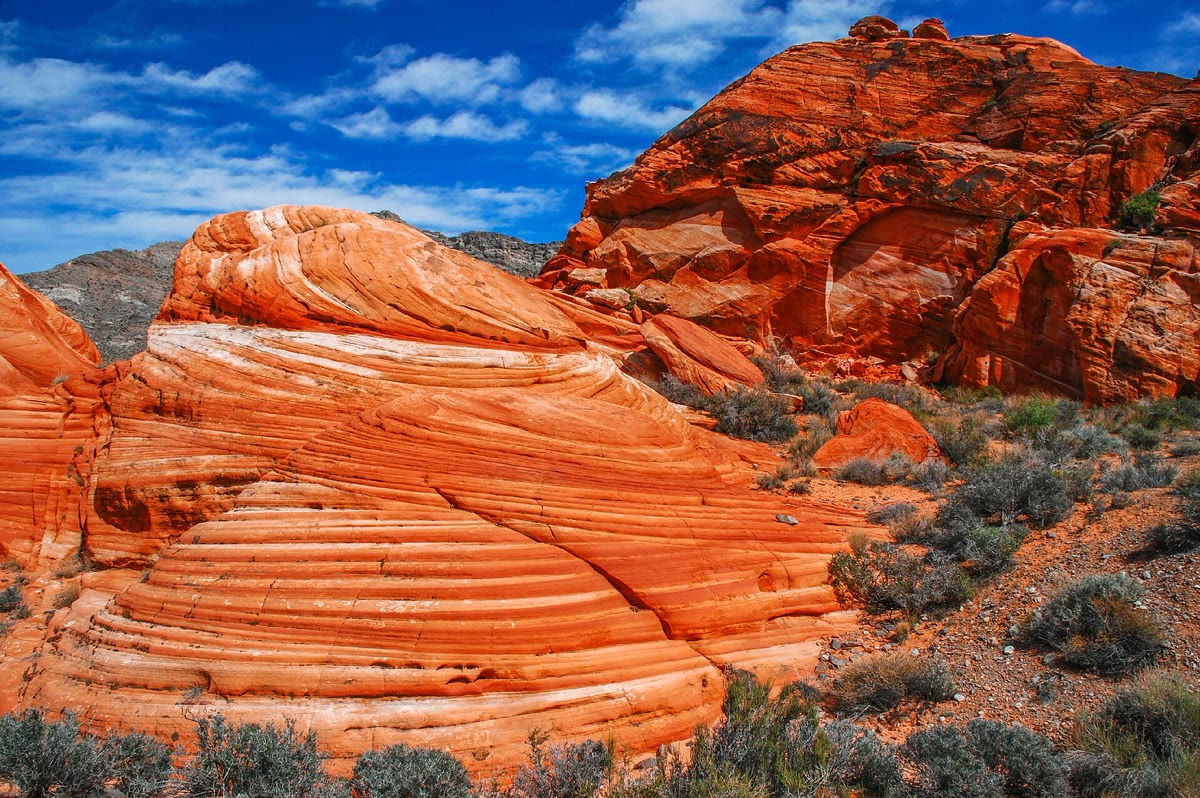
\includegraphics[height=3.6cm]{images/book3/b1-cross-bedding-aztec.jpg}};
\end{tikzpicture}

{\small बाएँ: आरोही तल-आकृतियों की ज्यामिति (योजनाबद्ध, कोण बढ़ा-चढ़ाकर)। गर्त आरोहण-कोण $\theta$ पर झुके सीधे पथों पर चलते हैं (मोटी रेखाएँ); उनमें से दो के बीच अग्र-परतों के निचले भाग मोटाई $T = L\sin\theta$ के समुच्चयों में संरक्षित हैं। दाएँ: नेवादा के मडी माउंटेन्स में एज़्टेक बालुकाश्म में \omterm{def:b1:clastic-sediments:cross-bedding}{तिर्यक-परत}: झुके समुच्चय पटलों के, जिनमें से हर एक शीर्ष पर अगली अपरदन-सतह से कटा है। फ़ोटो: Chip Carroon, Bureau of Land Management, CC~BY-SA~2.0, विकिमीडिया कॉमन्स के माध्यम से।}
\label{fig:b1:clastic-sediments:climb}
\end{omfigure}
% ledger: southard:climb, commons:aztec-crossbed

\emph{पुरा-धाराएँ।} एक बाहरी-भाग पर मापी तिर्यक-परतों की नति-दिशाएँ धारा की माध्य दिशा के चारों ओर बिखरती हैं, क्योंकि टीलों और लहरिकाओं के अग्र-पार्श्व मुड़े होते हैं, और स्वयं धाराएँ घूमती हैं। उनका माध्य सदिश-माध्य के रूप में लिया जाता है, अंकगणितीय के रूप में नहीं, उस कारण से जो \cref{prop:b1:field-lab-methods-1:vector-mean} में दिखाया गया है: दिगंश वृत्त पर कोण हैं, और 350 और 010 का माध्य 000 है, 180 नहीं।

\begin{proposition}[दिगंशों का माध्य]\label{prop:b1:clastic-sediments:azimuths}
मान लीजिए $\alpha_1, \ldots, \alpha_N$ दिगंश हैं, उत्तर से दक्षिणावर्त मापे गए। उनका सदिश माध्य $\bar\alpha$ और उनकी माध्य परिणामी लंबाई $\bar R$ इस प्रकार दिए गए हैं:
\[
  S = \sum_{i=1}^N \sin\alpha_i, \quad C = \sum_{i=1}^N \cos\alpha_i, \quad
  \bar\alpha = \operatorname{atan2}(S, C), \quad \bar R = \frac{\sqrt{S^2 + C^2}}{N},
\]
जहाँ $\operatorname{atan2}(S, C)$ वह कोण है जिसकी ज्या और कोज्या $S$ और $C$ के समानुपाती हैं, \ang{0} और \ang{360} के बीच लिया गया। $\bar R$ 0 और 1 के बीच है, और 1 केवल तभी है जब सारे दिगंश बराबर हों।
\end{proposition}

\begin{proof}
दिगंश $\alpha$ का इकाई सदिश, पूर्व को पहले निर्देशांक और उत्तर को दूसरे के रूप में लेकर, $(\sin\alpha, \cos\alpha)$ है। $N$ इकाई सदिशों का योग
$(S, C)$ है, और उसकी दिशा, सदिश माध्य (\cref{def:b1:field-lab-methods-1:mean-orientation}), का वह दिगंश है जिसकी ज्या और कोज्या $S/\sqrt{S^2+C^2}$ और $C/\sqrt{S^2+C^2}$ हैं। त्रिभुज-असमिका से $N$ इकाई सदिशों के योग की लंबाई अधिकतम $N$ है, समानता केवल तभी जब वे सब एक ही दिशा में इंगित करें।
\end{proof}

\begin{method}[तिर्यक-परत से पुरा-धारा]\label{met:b1:clastic-sediments:palaeocurrent}
\begin{enumerate}
  \item हर समुच्चय पर, अग्र-परतों की \omterm{def:b1:geological-maps:attitude}{नति-दिशा} मापिए, ऐसी सतहें चुनकर जो उनकी वास्तविक \omterm{def:b1:geological-maps:attitude}{नति} दिखाएँ (या \omterm{def:b1:geological-maps:attitude}{स्ट्राइक} और \omterm{def:b1:geological-maps:attitude}{नति} मापिए)।
  \item मुख्य परतबंदी का \omterm{def:b1:geological-maps:attitude}{अभिविन्यास} मापिए; यदि वह कुछ अंशों से अधिक झुकी है, तो हर अग्र-परत को परतबंदी के \omterm{def:b1:geological-maps:attitude}{स्ट्राइक} के चारों ओर क्षैतिज पर घुमाइए (यह घुमाव तीसरे खंड के स्टीरियोग्राफ़िक प्रक्षेपण से होता है)।
  \item सुधारी गई नति-दिशाओं का सदिश माध्य $\bar\alpha$ और $\bar R$ परिकलित कीजिए (\cref{prop:b1:clastic-sediments:azimuths})।
  \item पाठनों को एक गुलाब-आरेख, दिगंशों का एक वृत्तीय हिस्टोग्राम, के रूप में आलेखित कीजिए, यह देखने के लिए कि वे एक समूह बनाते हैं या दो: ज्वारीय धाराएँ जो उलटती हैं, विपरीत दिशाओं में नत समुच्चय बनाती हैं, हेरिंगबोन \omterm{def:b1:clastic-sediments:cross-bedding}{तिर्यक-परत} में, और तब एक एकल माध्य निरर्थक होता है।
\end{enumerate}
\end{method}
% ledger: og:sorting-environments

\emph{अन्य संरचनाएँ।} कई अन्य संरचनाएँ निक्षेपण की परिस्थितियों और परतों की ऊपर की दिशा अभिलेखित करती हैं। एक \omterm{def:b1:clastic-sediments:turbidite}{क्रमित परत} ऊपर की ओर बारीक होती है, अपने आधार पर मोटे से ऊपर बारीक तक, जैसे कण घटती धारा से बैठते हैं, सबसे मोटे पहले (\cref{def:b1:clastic-sediments:turbidite})। कीचड़-दरारें, अपने ऊपर की परत से भरी सिकुड़न-दरारों के बहुभुज, वहाँ बनते हैं जहाँ कीचड़ हवा में सूखता है, जैसे ज्वारीय समतलों और बाढ़-मैदानों पर। धारा द्वारा नीचे की कीचड़ में काटे गए गर्त, और ऊपर की बालू से भरे, बालुकाश्म-परत के आधार पर साँचों के रूप में संरक्षित रहते हैं, और उनके आकार वह दिशा बताते हैं जिधर धारा गई।
% ledger: og:sorting-environments

\section{फ़ेसीज़, नदियाँ और डेल्टा}\label{sec:b1:clastic-sediments:rivers-deltas}

\omterm{def:b1:clastic-sediments:grain-size}{कण-आकार}, \omterm{def:b1:clastic-sediments:sorting}{छँटाव}, संरचनाएँ, जीवाश्म और संघटन मिलकर एक तलछटी शैल का चरित्र बनाते हैं, और भूवैज्ञानिक उस चरित्र के लिए एक ही शब्द प्रयोग करते हैं।

\begin{definition}[अवसादी फ़ेसीज़, निक्षेपण-परिवेश]\label{def:b1:clastic-sediments:facies}
एक \emph{अवसादी फ़ेसीज़}\index{अवसादी फ़ेसीज़} तलछटी शैल का एक पिंड है जो अपनी शैल-विज्ञान, \omterm{def:b1:clastic-sediments:grain-size}{कण-आकार}, अवसादी संरचनाओं और जीवाश्मों से दूसरों से भिन्न है, जो सब उन परिस्थितियों को दर्शाते हैं जिनमें वह बना। \emph{निक्षेपण-परिवेश}\index{निक्षेपण-परिवेश} वह स्थान है, अपनी भौतिक, रासायनिक और जैविक परिस्थितियों के साथ, जिसमें एक तलछट बिछाई जाती है: एक नदी की धारा, एक बाढ़-मैदान, एक तट, एक डेल्टा की ढलान, गहरे समुद्र का तल।
\end{definition}
% ledger: og:sorting-environments

एक फ़ेसीज़ एक विवरण है, एक परिवेश एक व्याख्या, और कई परिवेश एक ही फ़ेसीज़ बना सकते हैं: लहरिका-युक्त बालू नदियों में, ज्वारीय समतलों पर और गहरे समुद्र के तल पर बिछती है। इसलिए व्याख्या फ़ेसीज़ के समुच्चयों और उस क्रम पर टिकती है जिसमें वे जमे हैं, जो परिवेशों की दिक्-गति का अनुसरण करता है: उस जमाव के सामान्य नियम, और हर परिवेश के मानक प्रतिरूप, पुस्तक 5 के विषय हैं। यह अध्याय मुख्य खंडजात परिवेशों और उन ऊर्ध्वाधर उत्तराधिकारों का वर्णन करता है जो उन्हें पहचानते हैं।

\emph{गुंफित और विसर्पी नदियाँ।} नदियाँ दो मुख्य शैलियों में आती हैं। एक गुंफित नदी कई धाराओं में बहती है जो बजरी और बालू की पट्टियों के चारों ओर बँटती और मिलती हैं; गुंफित नदियाँ अपने उद्गम के निकट, पर्वतों के नीचे या हिमनदों के सामने, मोटे भार ढोती हैं, और उनके निक्षेप बजरी की चादरें और मोटी, तिर्यक-परतदार बालू हैं, कीचड़ थोड़ा। एक विसर्पी नदी एक ही टेढ़ी-मेढ़ी धारा में बहती है। सबसे तेज़ पानी हर मोड़ के बाहरी किनारे के साथ बहता है, जहाँ वह कटे तट को अपरदित करता है; भीतर की ओर, जहाँ पानी सबसे धीमा है, बालू बिंदु-पट्टी पर बिछती है। इस प्रकार विसर्पें बगल में खिसकती हैं, एक ओर अपरदन करती हैं और दूसरी ओर निर्माण; किनारों के पार बाढ़-मैदान केवल बाढ़ों की कीचड़ पाता है।
% ledger: og:rivers

बिंदु-पट्टी का क्रम तल-आकृतियों से निकलता है। पट्टी के पैर पर, सबसे गहरे और सबसे तेज़ पानी में, धारा सबसे मोटे कण छोड़ती है और टीले बनाती है; धीमी ढलान वाली पट्टी के ऊपर पानी उथला और धीमा होता है, बालू बारीक, और टीले लहरिकाओं को रास्ता देते हैं (\cref{sec:b1:clastic-sediments:bedforms}); शीर्ष पर पट्टी बाढ़-मैदान में बदल जाती है। जैसे-जैसे मोड़ खिसकता है, इनमें से हर क्षेत्र नीचे वाले पर खिसकता है, और निक्षेप में एक छेद उन्हें एक पर एक जमे पाता है: एक अपरदन-सतह से कीचड़ तक ऊपर की ओर बारीक होता क्रम, हर धारा-गुज़रने के लिए एक, जिसकी मोटाई उस धारा की गहराई के लगभग बराबर है।

\emph{डेल्टा।} जहाँ एक नदी एक स्थिर जल-राशि में प्रवेश करती है, उसकी धारा फैलती और धीमी होती है, और उसका भार गिराया जाता है: मुख के निकट मोटा भार, और आगे बारीक। एक डेल्टा आगे बढ़ता है, या अग्र-प्रसार करता है, जब तक नदी तलछट की उतनी आपूर्ति करती है जितनी लहरें और ज्वार बहा नहीं सकते। लहरें और ज्वार आपूर्ति के साथ जो करते हैं वही उसका आकार तय करता है।

\begin{definition}[नदी-प्रधान, तरंग-प्रधान और ज्वार-प्रधान डेल्टा]\label{def:b1:clastic-sediments:delta}
एक डेल्टा \emph{नदी-प्रधान}\index{नदी-प्रधान डेल्टा} होता है जब नदी की आपूर्ति लहरों और ज्वारों पर भारी पड़ती है, और उसकी वितरिका-धाराएँ, अपने ही प्राकारों से सीमित, समुद्र में बालू की लंबी उँगलियाँ बनाती हैं; वह \emph{तरंग-प्रधान}\index{तरंग-प्रधान डेल्टा} होता है जब लहरें मुखों तक लाई गई बालू को एक चिकने, मेहराबदार तट के साथ तट और तट-कटकों में फिर से काम करती हैं; वह \emph{ज्वार-प्रधान}\index{ज्वार-प्रधान डेल्टा} होता है जब मुखों के भीतर-बाहर बहती ज्वारीय धाराएँ उसकी बालू को प्रवाह के समांतर पट्टियों और कटकों में आकार देती हैं, कीप-आकार की धाराओं से अलग।
\end{definition}
% ledger: og:deltas

\begin{omfigure}
\begin{tikzpicture}[font=\footnotesize, >={Stealth[length=4pt]}]
% meander in plan view (schematic) and the fining-upward log of a point bar
\begin{scope}[yscale=0.8]
  \fill[green!8] (-0.2,-0.4) rectangle (7.2,4.4);
  \draw[omSea!80!black, line width=9pt] plot[smooth, tension=0.7] coordinates {(0,3.6) (1.4,3.7) (2.6,2.8) (2.3,1.4) (3.2,0.5) (4.6,0.8) (5.0,2.2) (5.6,3.4) (7.0,3.5)};
  \draw[omSea!45, line width=7pt] plot[smooth, tension=0.7] coordinates {(0,3.6) (1.4,3.7) (2.6,2.8) (2.3,1.4) (3.2,0.5) (4.6,0.8) (5.0,2.2) (5.6,3.4) (7.0,3.5)};
  % point bars (inside of bends) with scroll lines
  \foreach \r in {0.25,0.45,0.65} {\draw[brown!60!black, densely dotted] (3.45,1.15) ++(200:\r) arc[start angle=200, end angle=340, radius=\r];}
  \fill[brown!25, opacity=0.8] (3.45,1.25) ellipse[x radius=0.55, y radius=0.35];
  \node[align=center] at (3.45,1.95) {बिंदु-पट्टी\\ (निक्षेपण)};
  \fill[brown!25, opacity=0.8] (1.75,2.75) ellipse[x radius=0.4, y radius=0.45];
  \node[align=center] at (1.3,1.95) {बिंदु-पट्टी};
  \draw[red!60!black, thick] (2.9,0.2) .. controls (3.3,0.0) and (4.3,0.15) .. (4.85,0.6);
  \node[red!60!black, anchor=north] at (4.0,0.0) {कटा तट (अपरदन)};
  \draw[->, black!70] (5.9,3.0) -- (6.7,3.15) node[right] {प्रवाह};
  \node[anchor=north west, black!60] at (5.2,1.3) {बाढ़-मैदान};
  \node[font=\footnotesize] at (3.5,-0.85) {(क) एक विसर्पी, ऊपर से देखी गई};
\end{scope}
\begin{scope}[xshift=9.2cm, yshift=-0.3cm, yscale=0.8]
  % log: x width = grain size; y = height
  \draw[lith shale] (0,3.6) rectangle (0.8,4.6);
  \draw[lith sandstone] (0,2.6) rectangle (1.2,3.6);
  \draw[lith sandstone] (0,0.6) rectangle (1.7,2.6);
  \draw[lith conglomerate] (0,0) rectangle (2.2,0.6);
  \draw[very thick, red!60!black] (0,0) -- (2.2,0);
  % cross-bed symbols
  \foreach \y in {0.9,1.5,2.1} {\draw[black!70] (0.3,\y) .. controls (0.6,\y+0.05) and (0.9,\y+0.25) .. (1.2,\y+0.4);}
  \foreach \x in {0.2,0.5,0.8} {\draw[black!70] (\x,3.0) -- ++(0.12,0.1) -- ++(0.12,-0.1);}
  \node[anchor=west, align=left] at (2.4,4.1) {बाढ़-मैदान की कीचड़,\\ जड़ें, कीचड़-दरारें};
  \node[anchor=west, align=left] at (2.4,3.1) {बारीक बालू, लहरिका-\\ तिर्यक-पटलन};
  \node[anchor=west, align=left] at (2.4,1.6) {मध्यम से मोटी बालू,\\ टीला-तिर्यक-परत};
  \node[anchor=west, align=left] at (2.4,0.3) {अपरदन-सतह पर\\ बजरी का अवशेष};
  \draw[->] (-0.35,0) -- (-0.35,4.6) node[above] {ऊपर};
  \draw[<->, black!60] (-0.7,0) -- node[above, rotate=90, font=\scriptsize] {धारा की गहराई} (-0.7,3.6);
  \node[font=\footnotesize] at (1.8,-0.5) {(ख) बिंदु-पट्टी का क्रम};
\end{scope}
\end{tikzpicture}

{\small (क)~एक विसर्पी नदी (योजनाबद्ध): धारा हर मोड़ के बाहरी किनारे को अपरदित करती है और उसके भीतर की बिंदु-पट्टी पर बालू बिछाती है; वक्र विसर्पी रेखाएँ पट्टी की क्रमागत स्थितियाँ हैं। (ख)~एक प्रवासी बिंदु-पट्टी द्वारा छोड़ा क्रम, हर परत की चौड़ाई उसके \omterm{def:b1:clastic-sediments:grain-size}{कण-आकार} के समानुपाती (योजनाबद्ध)। वह ऊपर की ओर बारीक होता है, और उसकी मोटाई धारा की गहराई दर्शाती है।}
\label{fig:b1:clastic-sediments:point-bar}
\end{omfigure}
% ledger: og:rivers, southard:phase-diagram

तीनों अंत-सदस्य एक त्रिभुज के कोने हैं जिसमें कोई भी डेल्टा तीनों प्रक्रियाओं की सापेक्ष शक्ति से रखा जा सकता है। मिसिसिपी का चिड़िया-पैर डेल्टा, मेक्सिको की खाड़ी में अपनी लंबी उँगलियों के साथ (\cref{ch:b1:erosion-transport}), क्लासिक \omterm{def:b1:clastic-sediments:delta}{नदी-प्रधान डेल्टा} है; नील, तटों के अपने चिकने चाप के साथ, एक \omterm{def:b1:clastic-sediments:delta}{तरंग-प्रधान}; गंगा और ब्रह्मपुत्र का डेल्टा, विश्व का सबसे बड़ा, एक \omterm{def:b1:clastic-sediments:delta}{ज्वार-प्रधान}।
% ledger: og:deltas

\begin{omfigure}
\begin{tikzpicture}[font=\footnotesize]
% delta classification triangle (schematic) and the Lena delta from Landsat
\begin{scope}[yscale=0.82]
  \coordinate (R) at (2.6,4.5); \coordinate (W) at (0,0); \coordinate (T) at (5.2,0);
  \fill[omDef!8] (R) -- (W) -- (T) -- cycle;
  \draw[thick] (R) -- (W) -- (T) -- cycle;
  \node[above, align=center] at (R) {\textbf{नदी-प्रधान}\\ लंबी उँगलियाँ, प्राकार};
  \node[below, align=center] at (W) {\textbf{तरंग-प्रधान}\\ चिकने तट-कटक};
  \node[below, align=center] at (T) {\textbf{ज्वार-प्रधान}\\ प्रवाह के समांतर पट्टियाँ};
  \fill[omThm] (2.6,2.9) circle[radius=2pt] node[below=1pt] {मिसिसिपी};
  \fill[omThm] (0.75,0.4) circle[radius=2pt] node[above right=0pt] {नील};
  \fill[omThm] (4.4,0.4) circle[radius=2pt] node[above left=0pt, align=right] {गंगा--\\ ब्रह्मपुत्र};
\end{scope}
\node[anchor=south west, inner sep=0] at (7.2,-0.9) {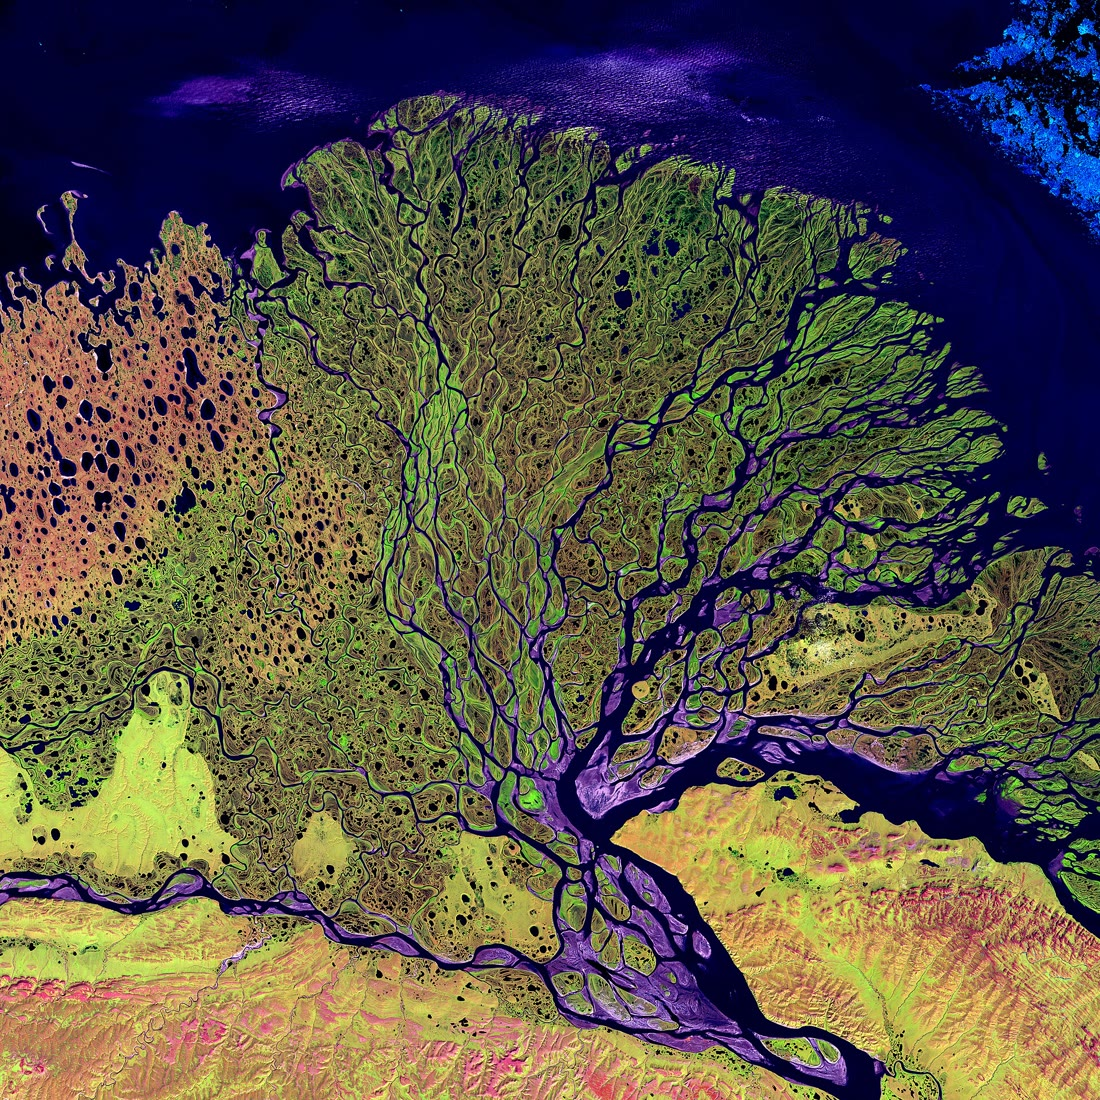
\includegraphics[height=5.2cm]{images/book3/b1-lena-delta.jpg}};
\end{tikzpicture}

{\small बाएँ: प्रक्रिया के अनुसार डेल्टा के तीन अंत-सदस्य (योजनाबद्ध; तीन उदाहरणों की स्थितियाँ सूचक हैं)। दाएँ: साइबेरिया में लीना का डेल्टा, लाप्तेव सागर में बना (ऊपर); नदी नीचे दाईं ओर से प्रवेश करती है और सैकड़ों वितरिकाओं में बँटती है। लैंडसैट~7 कूट-रंग चित्र, 27 फ़रवरी 2000। फ़ोटो: U.S. Geological Survey, सार्वजनिक क्षेत्र, विकिमीडिया कॉमन्स के माध्यम से।}
\label{fig:b1:clastic-sediments:deltas}
\end{omfigure}
% ledger: og:deltas, commons:lena-delta

\emph{उत्तरोत्तर-मोटा होता क्रम।} नदी-मुख के सामने, डेल्टा का एक मंद ढलान वाला मुख होता है, डेल्टा-मुख, जो समुद्र की ओर पूर्व-डेल्टा में बदलता है, जहाँ निलंबन से केवल कीचड़ बैठती है। जैसे-जैसे डेल्टा अग्र-प्रसार करता है, इनमें से हर क्षेत्र अपने सामने वाले पर आगे बढ़ता है: डेल्टा के मैदान पर एक छेद नीचे से ऊपर तक पूर्व-डेल्टा की परतदार कीचड़, फिर निचले डेल्टा-मुख की एकांतर गाद और बालू, फिर मुख-पट्टियों की तिर्यक-परतदार बालू पाता है, जो ऊपर से डेल्टा-मैदान की धाराओं से कटी हैं। यह क्रम ऊपर की ओर मोटा होता है, विसर्पी पट्टी का विलोम, और उसकी मोटाई उस पानी की गहराई के लगभग बराबर है जिसमें डेल्टा बना। उसकी दर डेल्टा-मुख की ज्यामिति से जुड़ी है।

\begin{proposition}[अग्र-प्रसार और संचय]\label{prop:b1:clastic-sediments:progradation}
मान लीजिए स्थिर ढलान $\alpha$ का एक डेल्टा-मुख, स्थिर समुद्र-तल पर, बिना आकार बदले वेग $v$ से क्षैतिज आगे बढ़ता है। मुख के नीचे का एक स्थिर बिंदु तब निक्षेप ऊर्ध्वाधर दर से प्राप्त करता है
\[
  a = v\,\tan\alpha,
\]
और मोटाई $h$ का डेल्टा-मुख क्रम वहाँ समय $h/(v\tan\alpha)$ में संचित होता है।
\end{proposition}

\begin{proof}
मुख $\mathrm dt$ समय में $v\,\mathrm dt$ आगे बढ़ता है। ढलान की सतह के नीचे एक स्थिर बिंदु पर, सतह मुख के दो बिंदुओं के बीच की ऊँचाई के अंतर से उठती है, जो क्षैतिज दूरी $v\,\mathrm dt$ पर हैं, अर्थात $v\,\mathrm dt\,\tan\alpha$, इसलिए दर। मुख उस बिंदु को पार करता है जब सतह $h$ उठती है, जिसमें समय $h/a$ लगता है।
\end{proof}

डेल्टा-मुख मंद ढलते हैं, इसलिए $\tan\alpha$ छोटा है: डेल्टा का मुख किसी भी बिंदु के नीचे तलछट के जमने से कहीं तेज़ आगे बढ़ता है (\cref{exo:b1:clastic-sediments:12})।

\begin{inthelab}[एक कोर का वर्णन]
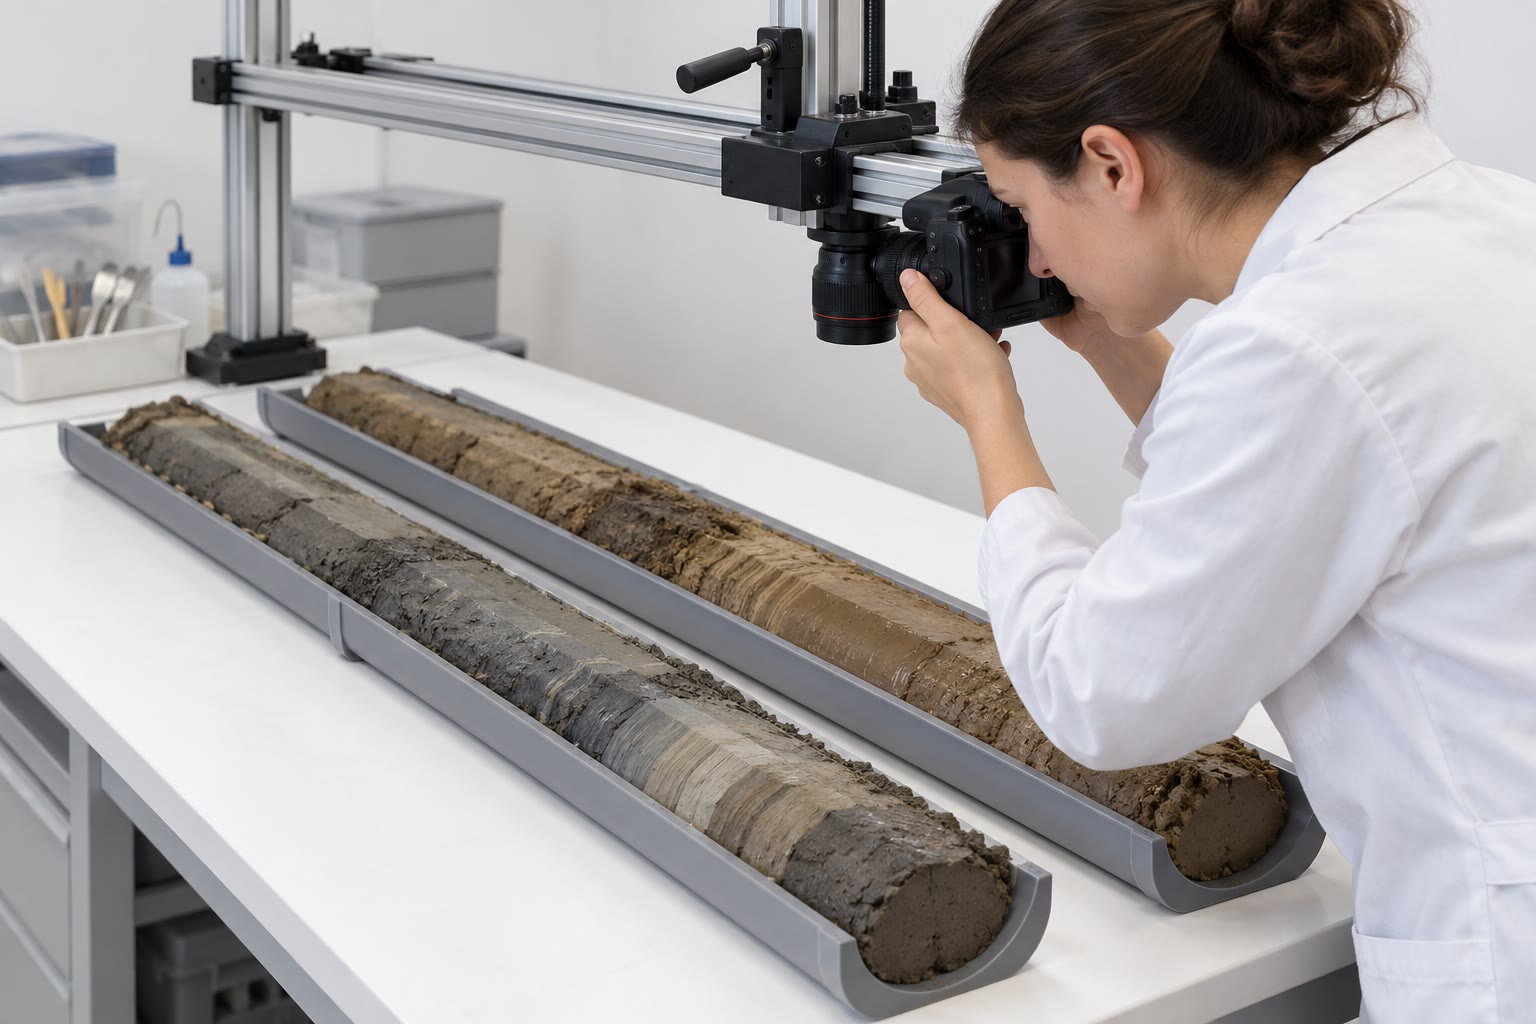
\includegraphics[width=0.3\linewidth]{images/book3/ai/b1-core-lab.jpg}\hfill
\begin{minipage}[b]{0.67\linewidth}
ड्रिल द्वारा ऊपर लाए तलछट या शैल के बेलन गहराई के क्रम में ट्रे में रखे जाते हैं, लंबाई में चीरे जाते हैं, और सूखने और रंग बदलने से पहले एकसमान प्रकाश में फ़ोटो खींचे जाते हैं। तब तलछट-वैज्ञानिक कोर का एक लॉग बनाता है, मीटर-दर-मीटर: शैल-विज्ञान, हर परत का \omterm{def:b1:clastic-sediments:grain-size}{कण-आकार} (स्तंभ की चौड़ाई), संरचनाएँ (\omterm{def:b1:clastic-sediments:cross-bedding}{तिर्यक-परत}, पटलन, क्रमण, बिल), \omterm{def:b1:geological-maps:geological-map}{संपर्क}, तीखे या क्रमिक, रंग और जीवाश्म। \omterm{def:b1:clastic-sediments:grain-size}{कण-आकार} विश्लेषण और पतले काटों के लिए नमूने लिए जाते हैं। एक कोर एक संकरी, एकल खिड़की है: तिर्यक-परतों की दिशा खो जाती है जब तक कोर अभिविन्यस्त न हो, और परतों का पार्श्व विस्तार अन्य छिद्रों से आना चाहिए।
\end{minipage}

\smallskip
{\small एक तलछट-प्रयोगशाला में फ़ोटो खींचने के लिए बिछाया गया एक कोर (AI से बनाया गया चित्र)।}
\end{inthelab}

\section{तट और शेल्फ़}\label{sec:b1:clastic-sediments:shoreline}

डेल्टाओं के बीच के तट पर, नदियों द्वारा लाई गई बालू लहरों और ज्वार से आकार पाती है। एक समुद्र-तट वह बालू है जिसे स्वैश, वह पतली पानी की चादर जो हर लहर टूटने के बाद उसके ऊपर-नीचे दौड़ती है, फिर से काम में लाती है: कण बार-बार हिलाए जाते हैं, बारीक तट से दूर बहा दिए जाते हैं, और तट की बालू सभी तलछटों में सबसे अच्छी छँटी और सबसे गोल होती है। स्वैश द्वारा बिछाए उनके परत समुद्र की ओर मंद झुकते हैं। कई नीचे तटों पर बालू अवरोधक द्वीप बनाती है, तट और पवन-उड़ी टीलों के लंबे कटक, जो मुख्य भूमि से लैगूनों द्वारा अलग हैं, शांत और बारीक-कण, ज्वारीय मुखों द्वारा समुद्र से जुड़े।

जहाँ ज्वार प्रबल और लहरें दुर्बल हैं, तट ज्वारीय समतलों से घिरा होता है, जो दिन में दो बार ढँके और उघड़ते हैं। वे निम्न-ज्वार रेखा के निकट बालू से, जहाँ धाराएँ सबसे प्रबल हैं, उच्च-ज्वार रेखा के निकट कीचड़ तक क्रमशः बदलते हैं, जहाँ शांत पानी मृत्तिका को बैठने देता है; उनके निक्षेप उलटी धारा को हेरिंगबोन \omterm{def:b1:clastic-sediments:cross-bedding}{तिर्यक-परत} में, सूखने को कीचड़-दरारों में, और धारा और शांत पानी के एकांतर को पतली, लहरिका-युक्त बालू पर कीचड़ की ढकी परतों में दर्शाते हैं।

तट से दूर, शेल्फ़ पर लहरें केवल एक गहराई तक झाड़ती हैं, जो लहरों के आकार के साथ बढ़ती है। उसके ऊपर बालू छँटती और सरकती है; उसके नीचे कीचड़ बैठती है, तूफ़ानों को छोड़कर, जब बड़ी लहरें गहराई तक पहुँचती हैं और बालू की चादरें बिछाती हैं जिनमें मंद लहरदार पटलन होती है, जिसे होमोक्की तिर्यक-स्तरण कहते हैं। एक शेल्फ़ का क्रम इसलिए अक्सर अच्छे-मौसम की कीचड़ और तूफ़ानी बालू के एकांतर से बनता है, जो तट की ओर मोटी और मोटी होती जाती है।
% ledger: og:sorting-environments, folk:maturity

\section{गहरे-समुद्र के खंडजात}\label{sec:b1:clastic-sediments:deep-sea}

बालू और बजरी गहरे महासागरों के तलों तक भी पहुँचते हैं, हज़ारों मीटर नीचे और भूमि से सैकड़ों किलोमीटर दूर, और वे वहाँ ऐसे प्रवाहों द्वारा ढोए जाते हैं जिन्हें किसी ने पूरी तरह नहीं देखा: सघन, तलछट-भरी धाराएँ जो महाद्वीपीय ढलान से नीचे, महासागर के स्वच्छ पानी के नीचे बहती हैं।

\begin{history}[1929 में समुद्र-तल पर केबल]
18 नवंबर 1929 को न्यूफ़ाउंडलैंड के दक्षिण में, ग्रैंड बैंक्स के दक्षिणी किनारे के साथ, महाद्वीपीय ढलान पर परिमाण 7.2 के आघूर्ण वाला भूकंप आया। लगभग \qty{200}{km^3} तलछट ढलान पर खिसका, और एक सुनामी ने न्यूफ़ाउंडलैंड के तट पर 28 लोगों को मार डाला। समुद्र-तल के आर-पार बिछे बारह टेलीग्राफ़ केबल टूट गए, कुछ कई स्थानों पर। उपरिकेंद्र के निकट वाले तुरंत टूटे; बाकी, दक्षिण में और गहरे, अगले घंटों में एक-एक करके टूटे, ढलान के नीचे दूरी के क्रम में। 1952 में ब्रूस हीज़न और मॉरिस ईविंग ने टूटने के समय का अध्ययन करते हुए उसकी व्याख्या की: खिसकाव एक \omterm{def:b1:clastic-sediments:turbidite}{गंदलाव-धारा} में बदल गया था जो ढलान से नीचे और अतल मैदान के पार 480\,मील से अधिक तक बही, हर केबल को गुज़रते हुए तोड़ती। समय और दूरियों से उन्होंने उसकी गति का अनुमान लगाया: महाद्वीपीय उत्थान के ऊपरी भाग पर लगभग 50 नॉट, जहाँ ढलान लगभग \qty{0.5}{\percent} है, और अंतिम केबल पर, उसके उद्गम से लगभग 400 मील दूर, अब भी 12 नॉट। धीमी होते हुए, उन्होंने तर्क दिया, उसने मैदान पर एक \omterm{def:b1:clastic-sediments:turbidite}{क्रमित परत} बिछाई होगी, ऊपर की ओर बारीक होती हुई।
\end{history}
% ledger: nrcan:grand-banks, he52:grand-banks

पचास नॉट \qty{25.7}{m.s^{-1}} है, \qty{90}{km.h^{-1}} से अधिक, मुख्य सड़क पर एक कार की गति; 12 नॉट \qty{6.2}{m.s^{-1}} है; और 480 मील लगभग \qty{770}{km} हैं। टूटनों ने उस प्रवाह की पहली मापी गई गतियाँ भी दीं जो केवल उसके निक्षेपों से और टंकियों के प्रयोगों से अनुमानित हुआ था।
% ledger: he52:grand-banks

\begin{definition}[गंदलाव-धारा, गंदलाव-निक्षेप, क्रमित परत]\label{def:b1:clastic-sediments:turbidite}
एक \emph{गंदलाव-धारा}\index{गंदलाव-धारा} पानी की एक धारा है जिसे उसके निलंबन में रखे तलछट ने उसके चारों ओर के पानी से सघन बना दिया है, जो उस पानी के नीचे एक ढलान से नीचे बहती है, उसके कण उस प्रक्षोभ से निलंबन में रखे गए जो उसकी अपनी गति बनाती है। एक \emph{गंदलाव-निक्षेप}\index{गंदलाव-निक्षेप} एक गंदलाव-धारा का निक्षेप है। एक \emph{क्रमित परत}\index{क्रमित परत} एक ऐसी परत है जिसका \omterm{def:b1:clastic-sediments:grain-size}{कण-आकार} उसके आधार से शीर्ष तक घटता है।
\end{definition}
% ledger: og:sorting-environments, he52:grand-banks

एक \omterm{def:b1:clastic-sediments:turbidite}{गंदलाव-धारा} स्वयं को चलाती है: वह इसलिए चलती है कि उसका निलंबन भारी है, और वह अपना निलंबन इसलिए रखती है कि वह चलती है। एक तीखी ढलान पर वह तल से और तलछट उठा सकती है, सघन और तेज़ हो सकती है; अतल मैदान की मंद ढलान पर वह धीमी होती है, अपना भार गिराती है और समाप्त होती है।

\begin{proposition}[गंदलाव-धारा की गति]\label{prop:b1:clastic-sediments:turbidity}
मोटाई $h$ और घनत्व $\rho + \Delta\rho$ की एक \omterm{def:b1:clastic-sediments:turbidite}{गंदलाव-धारा} ढलान $S$ से घनत्व $\rho$ के जल के नीचे स्थिर रूप से बहती है। यदि तल और ऊपर के जल का प्रतिरोध प्रति इकाई क्षेत्रफल $\tau = \rho\,C_f\,U^2$ है, जहाँ $C_f$ एक विमाहीन घर्षण-गुणांक है, तो उसका माध्य वेग है
\[
  U = \sqrt{\frac{\Delta\rho}{\rho}\,\frac{g\,h\,S}{C_f}} .
\]
\end{proposition}

\begin{proof}
प्रमाण वही है जो गहराई-ढाल गुणनफल का है (\cref{prop:b1:erosion-transport:depth-slope}), भार को अतिरिक्त भार से बदलकर। धारा का इकाई क्षेत्रफल का एक स्तंभ $(\rho +
\Delta\rho) g h$ भारी है, और उसके विस्थापित जल का भार $\rho g h$: आसपास के पानी में केवल अतिरिक्त $\Delta\rho\,g\,h$ उसे ढलान से नीचे खींचता है, उसके अनुदिश घटक $\Delta\rho\,g\,h\,S$ के साथ। स्थिर प्रवाह में यह प्रतिरोध $\rho C_f U^2$ से संतुलित होता है, इसलिए $U^2 = (\Delta\rho/\rho)\,g\,h\,S/C_f$।
\end{proof}

प्रतिरोध-नियम $\tau = \rho C_f U^2$, वेग में द्विघाती, जलविज्ञान में प्रक्षुब्ध प्रवाहों का है (भौतिकी की पुस्तकें), और $C_f$ प्रयोग से मिलता है। सूत्र उस जल की उपेक्षा करता है जिसे धारा अपने ऊपरी पृष्ठ से अपने भीतर मिलाती है, जो उसे तनु और धीमा करता है। यह तीन कारकों की भूमिका दिखाता है: दुगुनी मोटाई, या दुगुने घनत्व, या दुगुने ढलान वाली धारा $\sqrt 2$ गुना तेज़ बहती है। एक निलंबन जिसके आयतन का भाग $c$ क्वार्ट्ज-कण हैं, उसका $\Delta\rho/\rho = 1.65\,c$ है (\cref{sec:b1:erosion-transport:settling}), जो छोटा है जब तक प्रवाह बहुत सांद्र न हो; यहीं \omterm{def:b1:clastic-sediments:turbidite}{गंदलाव-धारा} नदी से भिन्न है, जिसमें पानी का पूरा भार, छोटा अतिरिक्त नहीं, प्रवाह को चलाता है। 1929 के 50 नॉट पर आधे प्रतिशत ढलान पर चलने के लिए एक \omterm{def:b1:clastic-sediments:turbidite}{गंदलाव-धारा} को मोटाई और घनत्व-अतिरेक का एक बड़ा गुणनफल चाहिए (\cref{exo:b1:clastic-sediments:11})।

\emph{बूमा अनुक्रम।} 1962 में आर्नल्ड बूमा ने प्राचीन गहरे-समुद्र के अनुक्रमों के बालुकाश्म-परतों का आंतरिक क्रम पाँच विभागों में वर्णित किया, आधार से ऊपर अक्षरों से अंकित। A: अखंड या क्रमित बालू, प्रायः एक क्षरणकारी आधार पर; B: समांतर पटलन वाली बालू; C: लहरिका-तिर्यक-पटलन वाली बारीक बालू, प्रायः कुंचित; D: क्रमित होती पटलित गाद, कीचड़ में; E: कीचड़। यह क्रम एक अकेली घटती धारा का, एक बिंदु के ऊपर से गुज़रने का, अभिलेख माना जाता है: धीमी होती हुई वह पहले अपने सबसे मोटे कण एक साथ छोड़ती है, फिर एक ऊपरी समतल तल बनाती है, फिर लहरिकाएँ, फिर गाद और मृत्तिका बैठने देती है। पूरे अनुक्रम दुर्लभ हैं: ऊपरी विभाग अक्सर अगली धारा द्वारा अपरदित होते हैं, और स्रोत से दूर, जहाँ धारा दुर्बल है, निचले विभाग गायब होते हैं।
% ledger: og:sorting-environments, shanmugam:bouma

\begin{omfigure}
\begin{tikzpicture}[font=\footnotesize]
% Bouma sequence: log (schematic) and a labelled photograph
\begin{scope}
  \draw[lith shale] (0,4.0) rectangle (0.7,4.8);
  \draw[lith shale] (0,3.3) rectangle (0.9,4.0);
  \draw[lith sandstone] (0,2.2) rectangle (1.3,3.3);
  \draw[lith sandstone] (0,1.2) rectangle (1.6,2.2);
  \draw[lith sandstone] (0,0) rectangle (2.0,1.2);
  \draw[very thick, red!60!black] (0,0) .. controls (0.6,-0.12) and (1.4,0.1) .. (2.0,0);
  \foreach \y in {1.4,1.6,1.8,2.0} {\draw[black!70] (0.1,\y) -- (1.5,\y);}
  \foreach \x in {0.15,0.5,0.85} {\draw[black!70] (\x,2.55) .. controls (\x+0.12,2.75) .. (\x+0.3,2.6);}
  \foreach \y in {3.45,3.6,3.75,3.9} {\draw[black!60] (0.1,\y) -- (0.8,\y);}
  \foreach \x/\y in {0.4/0.3, 0.9/0.5, 1.4/0.25, 0.6/0.8, 1.2/0.9} {\fill[black!60] (\x,\y) circle[radius=0.06];}
  \node[anchor=west] at (2.2,4.4) {E \quad कीचड़};
  \node[anchor=west] at (2.2,3.65) {D \quad पटलित गाद से कीचड़};
  \node[anchor=west] at (2.2,2.75) {C \quad लहरिका-तिर्यक-पटलन};
  \node[anchor=west] at (2.2,1.7) {B \quad समांतर पटलन};
  \node[anchor=west] at (2.2,0.6) {A \quad क्रमित बालू};
  \node[anchor=west, red!60!black] at (2.2,-0.15) {क्षरणकारी आधार, तल-चिह्न};
  \draw[->] (-0.3,0) -- (-0.3,4.8) node[above] {ऊपर};
\end{scope}
\node[anchor=south west, inner sep=0] at (6.9,-0.3) {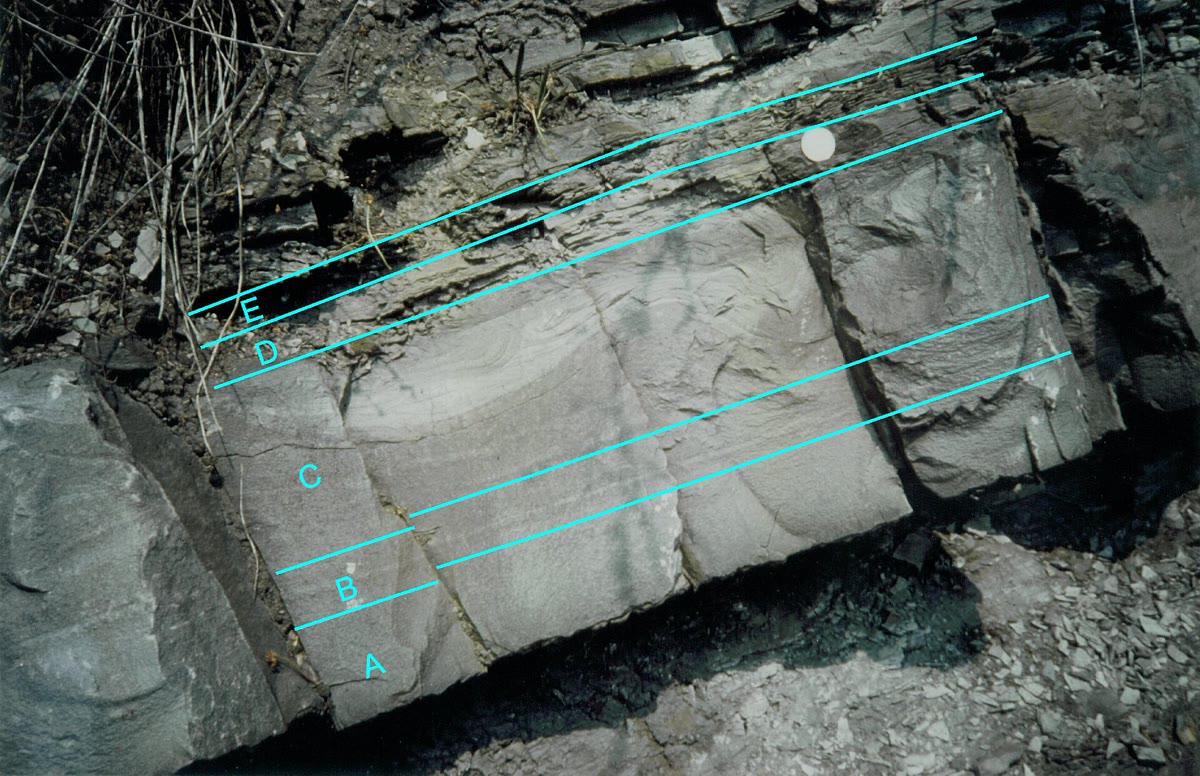
\includegraphics[height=5.2cm]{images/book3/b1-turbidite-bouma.jpg}};
\end{tikzpicture}

{\small बाएँ: बूमा अनुक्रम के पाँच विभाग, हर एक की चौड़ाई उसके \omterm{def:b1:clastic-sediments:grain-size}{कण-आकार} के समानुपाती (योजनाबद्ध)। दाएँ: जर्मनी में बेके-ओएज़े के ऊपरी डेवोनियन का एक \omterm{def:b1:clastic-sediments:turbidite}{गंदलाव-निक्षेप}, जिसके विभाग A से E तक फ़ोटोग्राफ़र ने अंकित किए; सिक्का पैमाना देता है। फ़ोटो: Jo Weber, CC~BY-SA~3.0, विकिमीडिया कॉमन्स के माध्यम से।}
\label{fig:b1:clastic-sediments:bouma}
\end{omfigure}
% ledger: og:sorting-environments, shanmugam:bouma, commons:bouma-becke-oese

बूमा अनुक्रम \omterm{def:b1:clastic-sediments:turbidite}{गंदलाव-निक्षेप} का मानक प्रतिरूप बन गया, और हज़ारों प्राचीन गहरे-समुद्र के बालुकाश्म उसके साथ व्याख्यायित हुए। व्याख्या विवादित है: ढलान के साथ बहती धाराएँ, गहरी ज्वारीय धाराएँ और आंतरिक तरंगें भी लहरिका-युक्त और पटलित बालू बनाती हैं, और कुछ अवसादविज्ञानी तर्क देते हैं कि कई परतें जिन्हें \omterm{def:b1:clastic-sediments:turbidite}{गंदलाव-निक्षेप} पढ़ा गया, उनमें प्रारूप-क्षेत्र की कुछ भी शामिल है, दूसरे प्रवाहों से बिछी थीं। आधुनिक महासागर में कुछ ही गंदलाव-धाराएँ देखी गई हैं, जबकि प्राचीन \omterm{def:b1:clastic-sediments:turbidite}{गंदलाव-निक्षेप} हज़ारों में गिने जाते हैं।
% ledger: shanmugam:bouma

सभी गहरे-समुद्र के खंडजात गंदलाव नहीं हैं। समोच्च-धाराएँ, मंद, गहरी धाराएँ जो महाद्वीपीय ढलान के समोच्चों का अनुसरण करती हैं, ढलान के तलछट को चिकने, लंबे विस्तारों में, समोच्च-निक्षेपों में, फिर से काम करती हैं। और महाद्वीपों से दूर, जहाँ न गंदलाव-धाराएँ पहुँचती हैं न समोच्च-धाराएँ, समुद्र-तल को केवल वही मिलता है जो ऊपर के पानी से बैठता है: प्लवकों के खोल और सबसे बारीक पवन-उड़ी धूल, अगले अध्याय के पेलेजिक तलछट (\cref{ch:b1:chemical-biogenic-sediments})।
% ledger: og:sorting-environments

\section{अभ्यास}

\begin{exercise}[$\star$]\label{exo:b1:clastic-sediments:1}
\qty{0.18}{mm}, \qty{0.75}{mm}, \qty{3}{mm}, \qty{0.012}{mm} और \qty{150}{mm} व्यासों को फ़ाई इकाइयों में, दो दशमलव तक, बदलिए, और हर एक का वर्ग बताइए (\cref{tab:b1:clastic-sediments:classes})।
% ledger: folk:wentworth-classes
\end{exercise}

\begin{exercise}[$\star$]\label{exo:b1:clastic-sediments:2}
एक नदी-बालू का संचयी वक्र $\varphi_5 = 0.62$, $\varphi_{16} =
1.05$, $\varphi_{50} = 1.71$, $\varphi_{84} = 2.43$ और $\varphi_{95} = 2.98$ देता है। उसका आलेखीय माध्य, फ़ाई इकाइयों में और मिलीमीटर में, और उसका समावेशी आलेखीय मानक विचलन परिकलित कीजिए, और उसका आकार और \omterm{def:b1:clastic-sediments:sorting}{छँटाव} बताइए।
% ledger: folk:graphic-measures, folk:sorting-classes
\end{exercise}

\begin{exercise}[$\star$]\label{exo:b1:clastic-sediments:3}
एक \qty{2}{cm} ऊँची \omterm{def:b1:clastic-sediments:bedform}{लहरिका} क्वार्ट्ज-बालू के तल पर \num{0.4} सरंध्रता वाली \qty{1}{cm} प्रति मिनट से प्रवास करती है। \cref{prop:b1:clastic-sediments:migration} से, प्रति इकाई चौड़ाई \omterm{def:b1:erosion-transport:load}{तल-भार} का आयतन, \si{m^2.s^{-1}} में, और एक दिन में एक मीटर शिखर पर ढोए गए क्वार्ट्ज ($\qty{2650}{kg.m^{-3}}$) का द्रव्यमान परिकलित कीजिए।
% ledger: hom:quartz
\end{exercise}

\begin{exercise}[$\star$]\label{exo:b1:clastic-sediments:4}
एक नॉट एक नॉटिकल मील, \qty{1852}{m}, प्रति घंटा है। (क)~1929 के \omterm{def:b1:clastic-sediments:turbidite}{गंदलाव-धारा} के लिए अनुमानित 50 और 12 नॉट की गतियों को मीटर प्रति सेकंड में बदलिए। (ख)~12 नॉट की धारा को \qty{100}{km} तय करने में कितना समय लगता है? (ग)~480 और 400 मील को किलोमीटर में बदलिए (एक मील \qty{1.609}{km} है)।
% ledger: he52:grand-banks
\end{exercise}

\begin{exercise}[$\star\star$]\label{exo:b1:clastic-sediments:5}
(क)~\cref{prop:b1:clastic-sediments:normal} के प्रमाण में दिए सामान्य वितरण के प्रतिशतकों का उपयोग करके, आलेखीय मानक विचलन $(\varphi_{84} - \varphi_{16})/2$ और अनुमान $(\varphi_{95} - \varphi_5)/3.3$ परिकलित कीजिए, उस सामान्य वितरण के लिए जिसका मानक विचलन $\sigma$ है। (ख)~एक वास्तविक तलछट के लिए दोनों क्यों भिन्न हो सकते हैं? कौन-सा प्रकार का तलछट उन्हें सबसे अधिक भिन्न करता है?
\end{exercise}

\begin{exercise}[$\star\star$]\label{exo:b1:clastic-sediments:6}
एक तिर्यक-लहरिका-निक्षेप में समुच्चय \qty{1.5}{cm} मोटे दिखाते हैं, उनकी सीमाओं के लंबवत मापे गए, \qty{15}{cm} अंतराल पर रखी लहरिकाओं से बने। (क)~आरोहण-कोण परिकलित कीजिए। (ख)~यदि लहरिकाएँ \qty{0.5}{cm} प्रति मिनट से चलतीं, तो तल किस दर से, सेंटीमीटर प्रति घंटे में, उठा? (ग)~ऐसी दर धारा के बारे में क्या बताती है?
% ledger: southard:climb
\end{exercise}

\begin{exercise}[$\star\star$]\label{exo:b1:clastic-sediments:7}
तिर्यक-परतों की छह नति-दिशाएँ, परतों की \omterm{def:b1:geological-maps:attitude}{नति} के लिए पहले से सुधारी गईं, 350, 020, 005, 340, 015 और 030 पढ़ी गईं। (क)~उनका अंकगणितीय माध्य परिकलित कीजिए। (ख)~उनका सदिश माध्य और $\bar R$ परिकलित कीजिए। (ग)~अंतर समझाइए।
\end{exercise}

\begin{exercise}[$\star\star$]\label{exo:b1:clastic-sediments:8}
तीन बालुकाश्म \omterm{def:b1:field-lab-methods-1:thin-section}{पतली काट} में जाँचे गए हैं। A में \qty{12}{\percent} मृत्तिका आधार और क्वार्ट्ज, फ़ेल्डस्पार और चट्टान-टुकड़ों के कोणीय कण हैं। B में \qty{2}{\percent} मृत्तिका, $\sigma_I = 0.40\,\varphi$ और फ़ोक के पैमाने पर \num{2.2} गोलाई के क्वार्ट्ज कण हैं। C में कोई मृत्तिका नहीं, $\sigma_I =
0.30\,\varphi$, \num{3.6} गोलाई के क्वार्ट्ज कण, और \qty{98}{\percent} क्वार्ट्ज हैं। हर एक की \omterm{def:b1:clastic-sediments:maturity}{संरचनात्मक परिपक्वता} बताइए, और हर एक के लिए निक्षेपण का एक परिवेश सुझाइए।
% ledger: folk:maturity
\end{exercise}

\begin{exercise}[$\star\star$]\label{exo:b1:clastic-sediments:9}
(क)~\qty{0.3}{m} गहरे \qty{1.5}{m.s^{-1}} पर बहते प्रवाह की, और \qty{2}{m} गहरी \qty{1.0}{m.s^{-1}} पर बहती नदी की फ़्रूड संख्या परिकलित कीजिए ($g
= \qty{9.81}{m.s^{-2}}$)। (ख)~\qty{1.5}{m.s^{-1}} का प्रवाह किस गहराई पर फ़्रूड संख्या 1 तक पहुँचेगा, और \qty{2}{m} गहरी नदी को कितना वेग चाहिए? (ग)~समुद्र-तट से बहते जल की चादरों में प्रतिलोम टीले क्यों आम हैं, और बड़ी नदियों में दुर्लभ?
% ledger: southard:ripples-dunes
\end{exercise}

\begin{exercise}[$\star\star\star$]\label{exo:b1:clastic-sediments:10}
बालू के एक छलनी-विश्लेषण से, पूरे-फ़ाई वर्गों में $-1$ से $5\,\varphi$ तक: 2, 8, 30, 40, 15 और 5 भार-प्रतिशत मिलते हैं। (क)~आघूर्ण-विधि से, फ़ाई इकाइयों में माध्य और मानक विचलन परिकलित कीजिए, और \omterm{def:b1:clastic-sediments:sorting}{छँटाव} का नाम दीजिए। (ख)~संचयी वक्र बनाइए, रैखिक अंतर्वेशन से $\varphi_5$, $\varphi_{16}$, $\varphi_{50}$, $\varphi_{84}$ और $\varphi_{95}$ पढ़िए, और $M_z$ और $\sigma_I$ परिकलित कीजिए। (ग)~तुलना कीजिए।
% ledger: folk:graphic-measures, folk:sorting-classes
\end{exercise}

\begin{exercise}[$\star\star\star$]\label{exo:b1:clastic-sediments:11}
\cref{prop:b1:clastic-sediments:turbidity} में $C_f = 0.003$ लीजिए। (क)~\qty{50}{m} मोटी एक \omterm{def:b1:clastic-sediments:turbidite}{गंदलाव-धारा}, \qty{2}{\percent} घनत्व-अतिरेक के साथ, \num{0.005} ढलान से नीचे बहती है: उसकी गति मीटर प्रति सेकंड में और नॉट में परिकलित कीजिए। (ख)~उसी ढलान पर 1929 के 50 नॉट देने वाला मोटाई और सापेक्ष घनत्व-अतिरेक का कौन-सा गुणनफल होगा? (ग)~(क) की वही धारा \num{0.001} ढलान पर पहुँचती है: यदि और कुछ न बदले, तो उसकी नई गति परिकलित कीजिए। उसके भार का क्या होता है?
% ledger: he52:grand-banks
\end{exercise}

\begin{exercise}[$\star\star\star$]\label{exo:b1:clastic-sediments:12}
एक नदी अपने डेल्टा को हर वर्ष \qty{50}{Mt} तलछट देती है, जिसका \qty{70}{\percent} \qty{100}{km} चौड़े एक डेल्टा-मुख पर बैठता है जो \qty{30}{m} गहरे पानी में बनता है। निक्षेप का थोक घनत्व \qty{2000}{kg.m^{-3}} है। (क)~वह हर वर्ष कितना आयतन जोड़ता है? (ख)~यदि यह आयतन मुख की चौड़ाई के साथ पानी की पूरी गहराई भरे, तो मुख कितनी तेज़ी से आगे बढ़ता है? (ग)~मुख के नीचे, \ang{0.5} डेल्टा-मुख ढलान के साथ, एक स्थिर बिंदु पर तलछट किस दर से जमता है, और उस बिंदु पर ऊपर की ओर मोटा होता क्रम कितने वर्षों में बनता है?
\end{exercise}

\section{समस्या: एक प्राचीन डेल्टा से कोर पढ़ना}

\begin{problem}[{सप्ताहांत समस्या --- एक प्राचीन डेल्टा में एक छेद, कण-आकार से उसकी नदियों की दिशा तक}]
\label{pb:b1:clastic-sediments:1}
% values: calc/ch21.py; the borehole, its beds, ages and readings are invented
एक छेद एक प्राचीन डेल्टा द्वारा बिछाए \qty{24}{m} बालुकाश्म और मडस्टोन को पार करता है। भूवैज्ञानिक आधार से ऊपर चार इकाइयों का वर्णन करता है, और हर एक का एक नमूना विश्लेषित करता है।

\smallskip
\begin{center}\small
\begin{tabular}{@{}llccccc@{}}
\hline
इकाई (आधार से गहराई) & विवरण & $\varphi_5$ & $\varphi_{16}$ & $\varphi_{50}$ & $\varphi_{84}$ & $\varphi_{95}$ \\
\hline
1 (0--8 m) & लेमिनेटेड भूरा मडस्टोन & 4.2 & 5.0 & 6.6 & 8.4 & 9.6 \\
2 (8--16 m) & एकांतर सिल्टस्टोन और बालुकाश्म & 1.9 & 2.4 & 3.4 & 4.6 & 5.5 \\
3 (16--21 m) & तिर्यक-परतदार बालुकाश्म & 0.9 & 1.25 & 1.8 & 2.35 & 2.7 \\
4 (21--24 m) & कंकरीला बालुकाश्म, क्षरणकारी आधार & $-1.8$ & $-0.8$ & 0.9 & 2.1 & 2.9 \\
\hline
\end{tabular}
\end{center}

\medskip
\noindent\textbf{भाग I --- कण-आकार।}
\begin{enumerate}
  \item हर इकाई का आलेखीय माध्य $M_z$, फ़ाई इकाइयों में और मिलीमीटर में, परिकलित कीजिए।
  \item हर इकाई का समावेशी आलेखीय मानक विचलन $\sigma_I$ परिकलित कीजिए।
  \item हर इकाई के माध्य का आकार-वर्ग और \omterm{def:b1:clastic-sediments:sorting}{छँटाव} का नाम बताइए।
  \item कौन-सी इकाई सबसे अच्छी छँटी है? एक मुख-पट्टी पूर्व-डेल्टा की कीचड़ से बेहतर क्यों छँटी होगी?
  \item $\varphi_{50}$ और $\varphi_{84}$ के बीच रैखिक अंतर्वेशन से, इकाई~1 में मृत्तिका-आकार के कणों ($8\,\varphi$ से बारीक) का प्रतिशत आँकिए। वह उन धाराओं के बारे में क्या कहता है जहाँ वह जमी?
  \item इकाई~4 का संचयी वक्र इतना फैला क्यों है, यद्यपि वह एक धारा-बालू है?
\end{enumerate}

\medskip
\noindent\textbf{भाग II --- क्रम।}
\begin{enumerate}[resume]
  \item इकाई~1 से इकाई~3 तक माध्य आकार कैसे बदलता है? क्या क्रम ऊपर की ओर बारीक होता है या मोटा?
  \item इकाइयों 1, 2 और 3 को एक डेल्टा के भागों के रूप में व्याख्यायित कीजिए। हर एक के जमते समय डेल्टा का कौन-सा क्षेत्र स्थल पर था?
  \item तीनों इकाइयों का जमाव डेल्टा की गति के बारे में क्या दिखाता है?
  \item डेल्टा कम से कम कितनी गहराई के पानी में बना, और क्यों?
  \item इकाई~4 का एक क्षरणकारी आधार है और वह इकाई~3 से मोटी है। उसकी व्याख्या कीजिए।
  \item क्या एक बिंदु-पट्टी वही क्रम देगी? समझाइए।
\end{enumerate}

\medskip
\noindent\textbf{भाग III --- डेल्टा कितनी तेज़ी से आगे बढ़ा?}
इकाई~1 के आधार पर और इकाई~2 के शीर्ष पर ज्वालामुखी राख की दो पतली परतें तिथित हैं; वे \num{4000}~वर्ष दूर हैं।
\begin{enumerate}[resume]
  \item दोनों राखों के बीच संचय की माध्य दर, मिलीमीटर प्रति वर्ष में, परिकलित कीजिए।
  \item डेल्टा-मुख \ang{0.5} पर ढला था। \cref{prop:b1:clastic-sediments:progradation} से, वह गति परिकलित कीजिए जिस पर वह आगे बढ़ा, मीटर प्रति वर्ष में।
  \item \num{4000}~वर्षों में मुख कितना आगे बढ़ा?
  \item इस दर पर, स्थल पर इकाइयों 1 से 3 के \qty{21}{m} जमने में कितना समय लगा?
  \item एक डेल्टा में संचय की दर हर जगह एक ही समय पर एक क्यों नहीं है?
\end{enumerate}

\medskip
\noindent\textbf{भाग IV --- नदियाँ किधर बहती थीं?}
इकाई~3 के तिर्यक-परतदार बालुकाश्म पर, एक निकटवर्ती बाहरी-भाग में जहाँ परतें क्षैतिज हैं, बारह अग्र-परत नति-दिशाएँ मापी जाती हैं: 352, 010, 025, 004, 338, 017, 031, 359, 012, 046, 006 और 344।
\begin{enumerate}[resume]
  \item बारह पाठनों का अंकगणितीय माध्य परिकलित कीजिए। क्या वह सार्थक है?
  \item \cref{prop:b1:clastic-sediments:azimuths} के योग $S$ और $C$ परिकलित कीजिए।
  \item माध्य परिणामी लंबाई $\bar R$ परिकलित कीजिए। क्या पाठन संगत हैं?
  \item डेल्टा किस सामान्य दिशा में बना, और भूमि कहाँ थी?
  \item यदि परतें झुकी हों, तो नति-दिशाओं को क्यों घुमाना चाहिए, और किस अक्ष के बारे में?
  \item क्या एक ज्वारीय धारा ने ये तिर्यक-परतें बनाई होंगी? उसका गुलाब-आरेख कैसा दिखेगा?
  \item निकटतम अंश तक, इकाई~3 के तिर्यक-परतदार बालुकाश्म की माध्य \omterm{def:b1:clastic-sediments:cross-bedding}{पुरा-धारा} दिगंश क्या है?
\end{enumerate}
\end{problem}
